%%
% ESAD
%
\infoleveqnull{\section{Detector Gas Supply System}
}
%%
%%
% Operations Manual
%
\infolevone{
\chapter[The Hall A Gas System]{The Hall A Gas System
\label{chap:hrs-det-gas}
}
\footnote{Authors: Chandan Ghosh \email{chandan@jlab.org}}
\section{Overview}
}
%%
Currently, the only gas requirement from the hall is for the GEM detectors for the SBS experiments. 
For the GEM detectors, an Ar-CO2 (75\%-25\%) mixture is required during production and testing, and nitrogen when the chambers are not in use and need to be purged. 
Ultra High Purity (99.999\%) grade gasses (Ar, N$_2$) and Colman grade (99.999\%) liquid CO$_2$ are used in the system for the safe operation of the GEM detectors. 
For purging the chambers with boil-off nitrogen, typically a 350 high-pressure dewar is used. 
Decidated gas mixing systems are used to mix the Ar and CO$_2$ to the desired ratio and binary gas analyzers (SRS-made BGA244) are used to ensure and monitor the mixing ratio. 
There are two gas systems that supplies gas for the GEM detectors --henceforth mentioned as old and new gas systems.

\section{The Old Gas System}
%\label{oldgassystem}
 This is a part of the gas system designed to supply gas for the HRS detectors. This old gas system is on the right side of the Hall A Truck ramp as one looks into the hall.
Figure~\ref{fig:oldsystemschematic} shows a schematic of the old gas system. The methane and ethane gas lines exist.
 But we DO NOT USE them and we have NO methane or ethane in the system.
\begin{figure}[h!]
\begin{center}
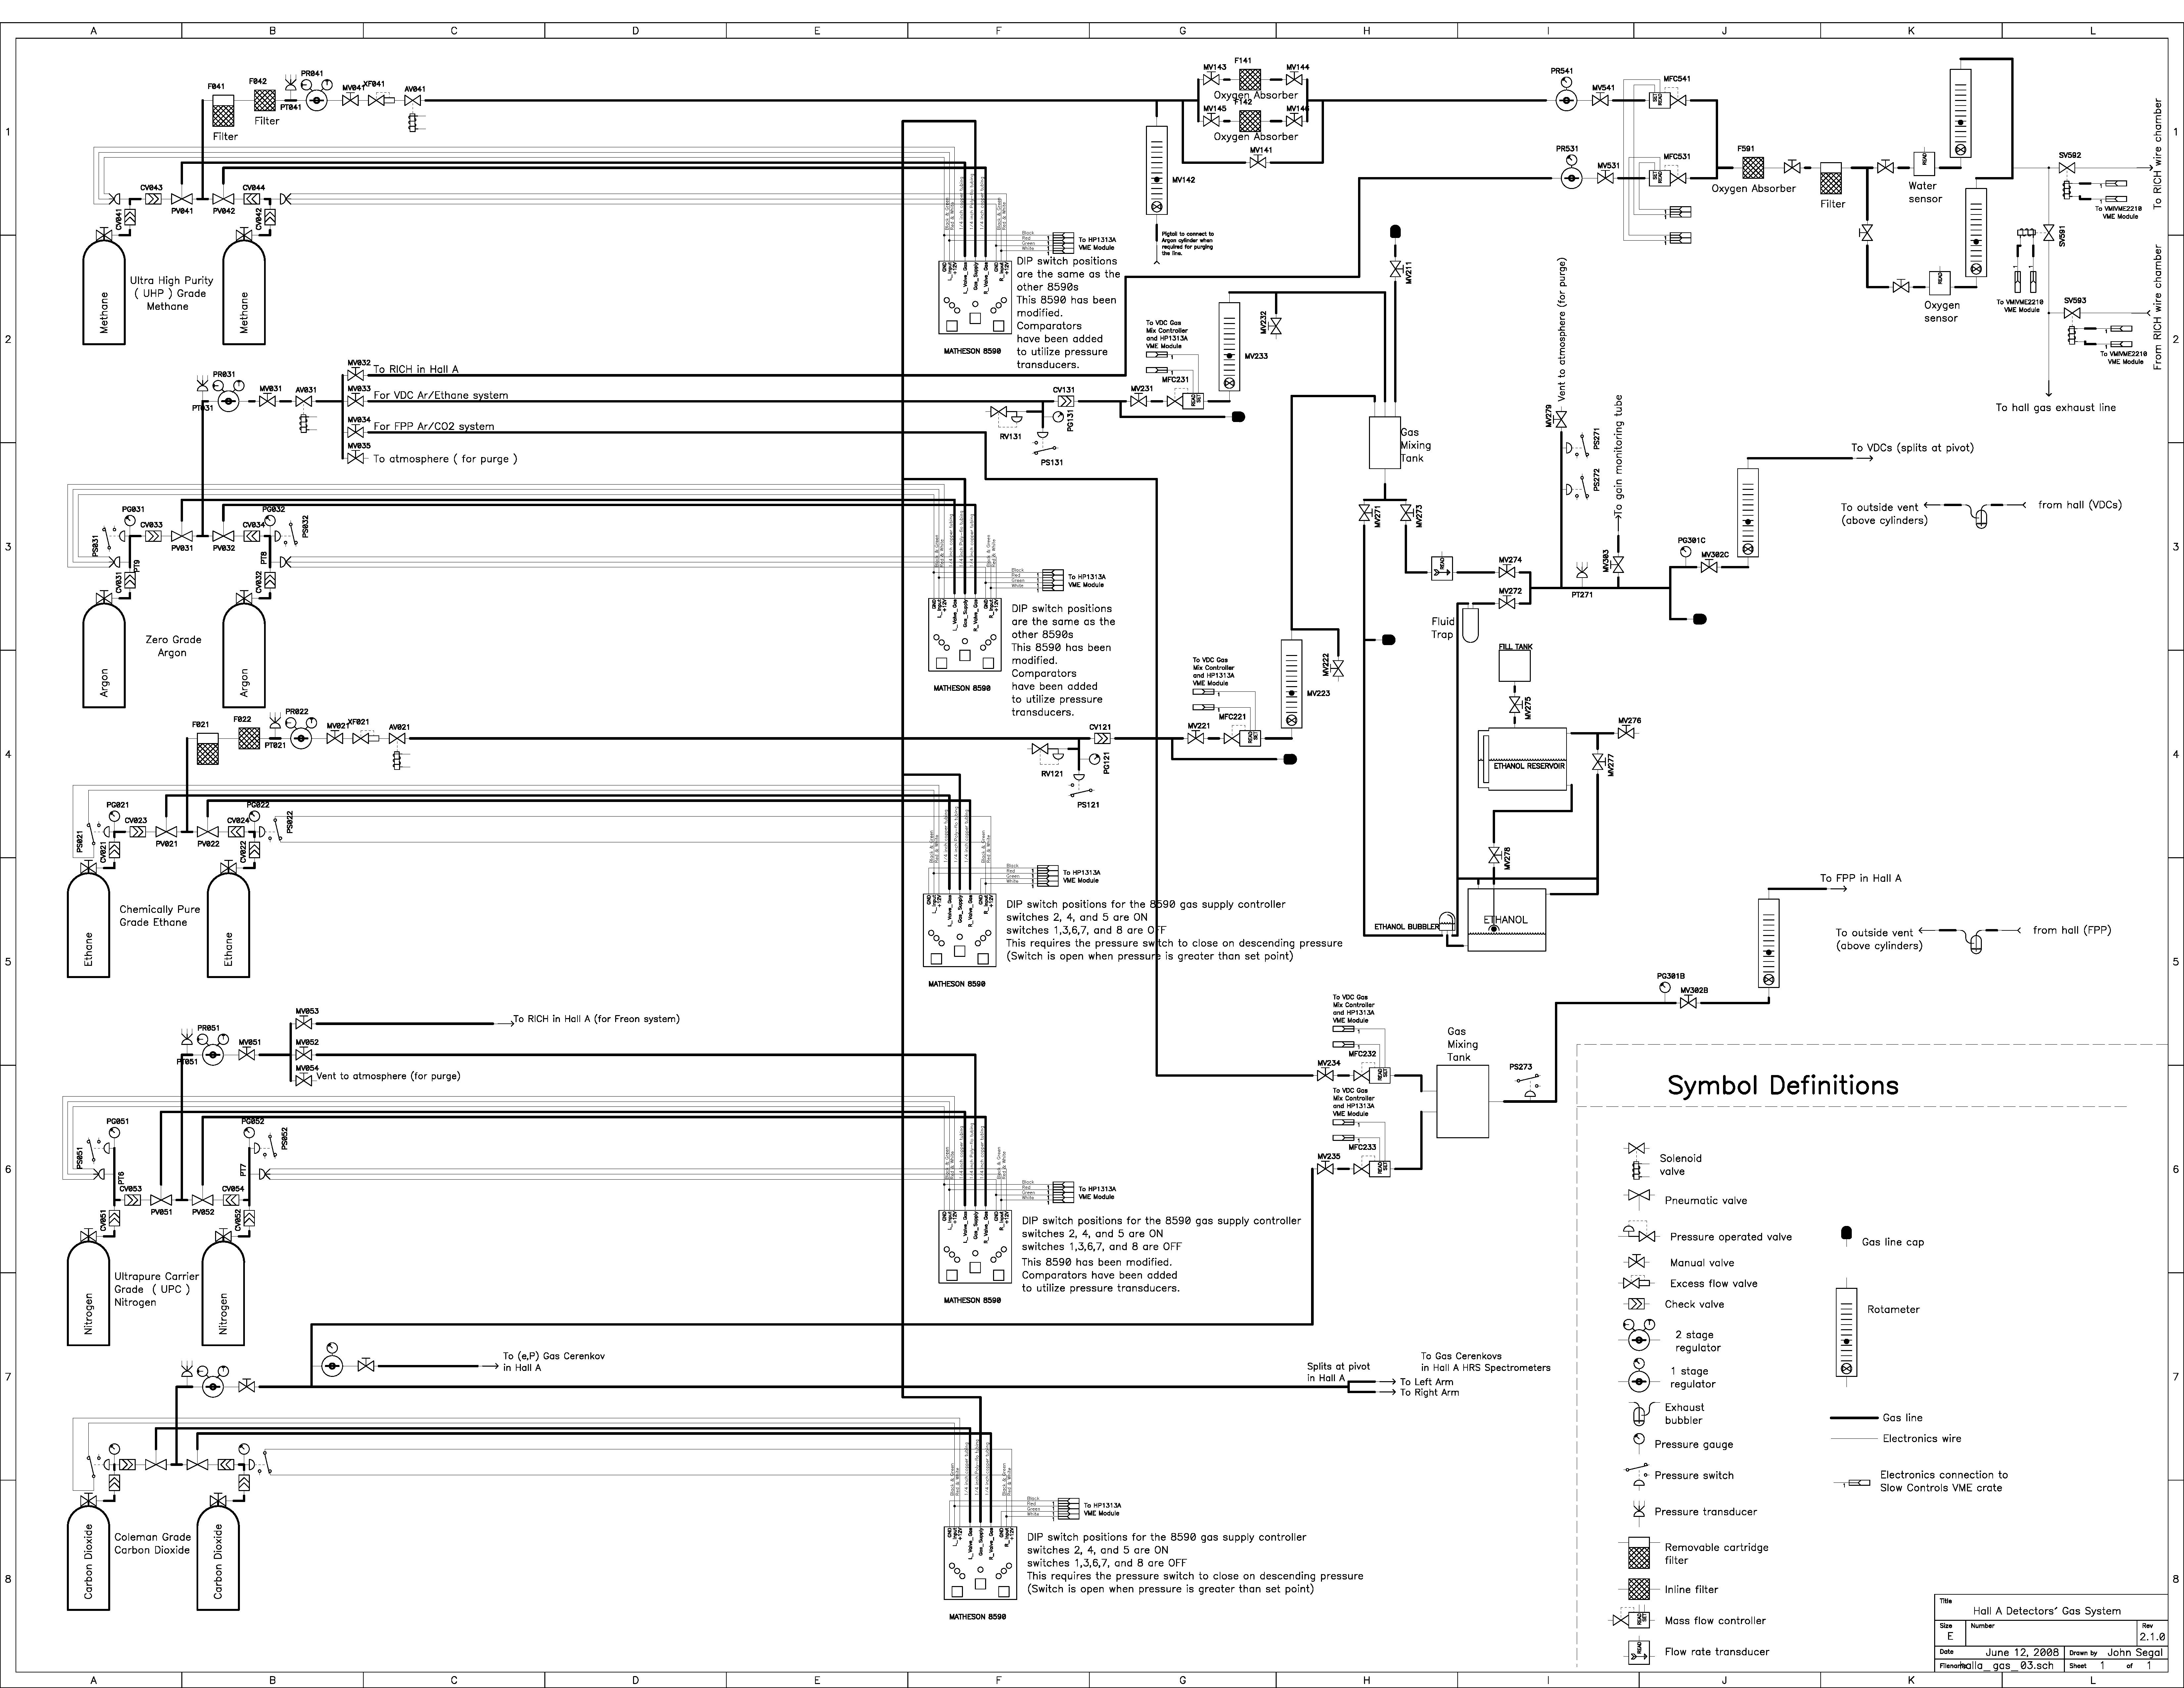
\includegraphics[angle=0,width=0.9\textwidth,clip]{gas_system_old.pdf}
\caption{The old gas system from the HRS era. Methane and Ethane lines exist, but we DO NOT have any methane or ethane in the system as we don't use them anymore. Currently, we are using part of the system that handles Ar, N$_2$, and CO$_2$ gases.}
\label{fig:oldsystemschematic}
\end{center}
\end{figure}
\begin{figure}[h]
\begin{center}
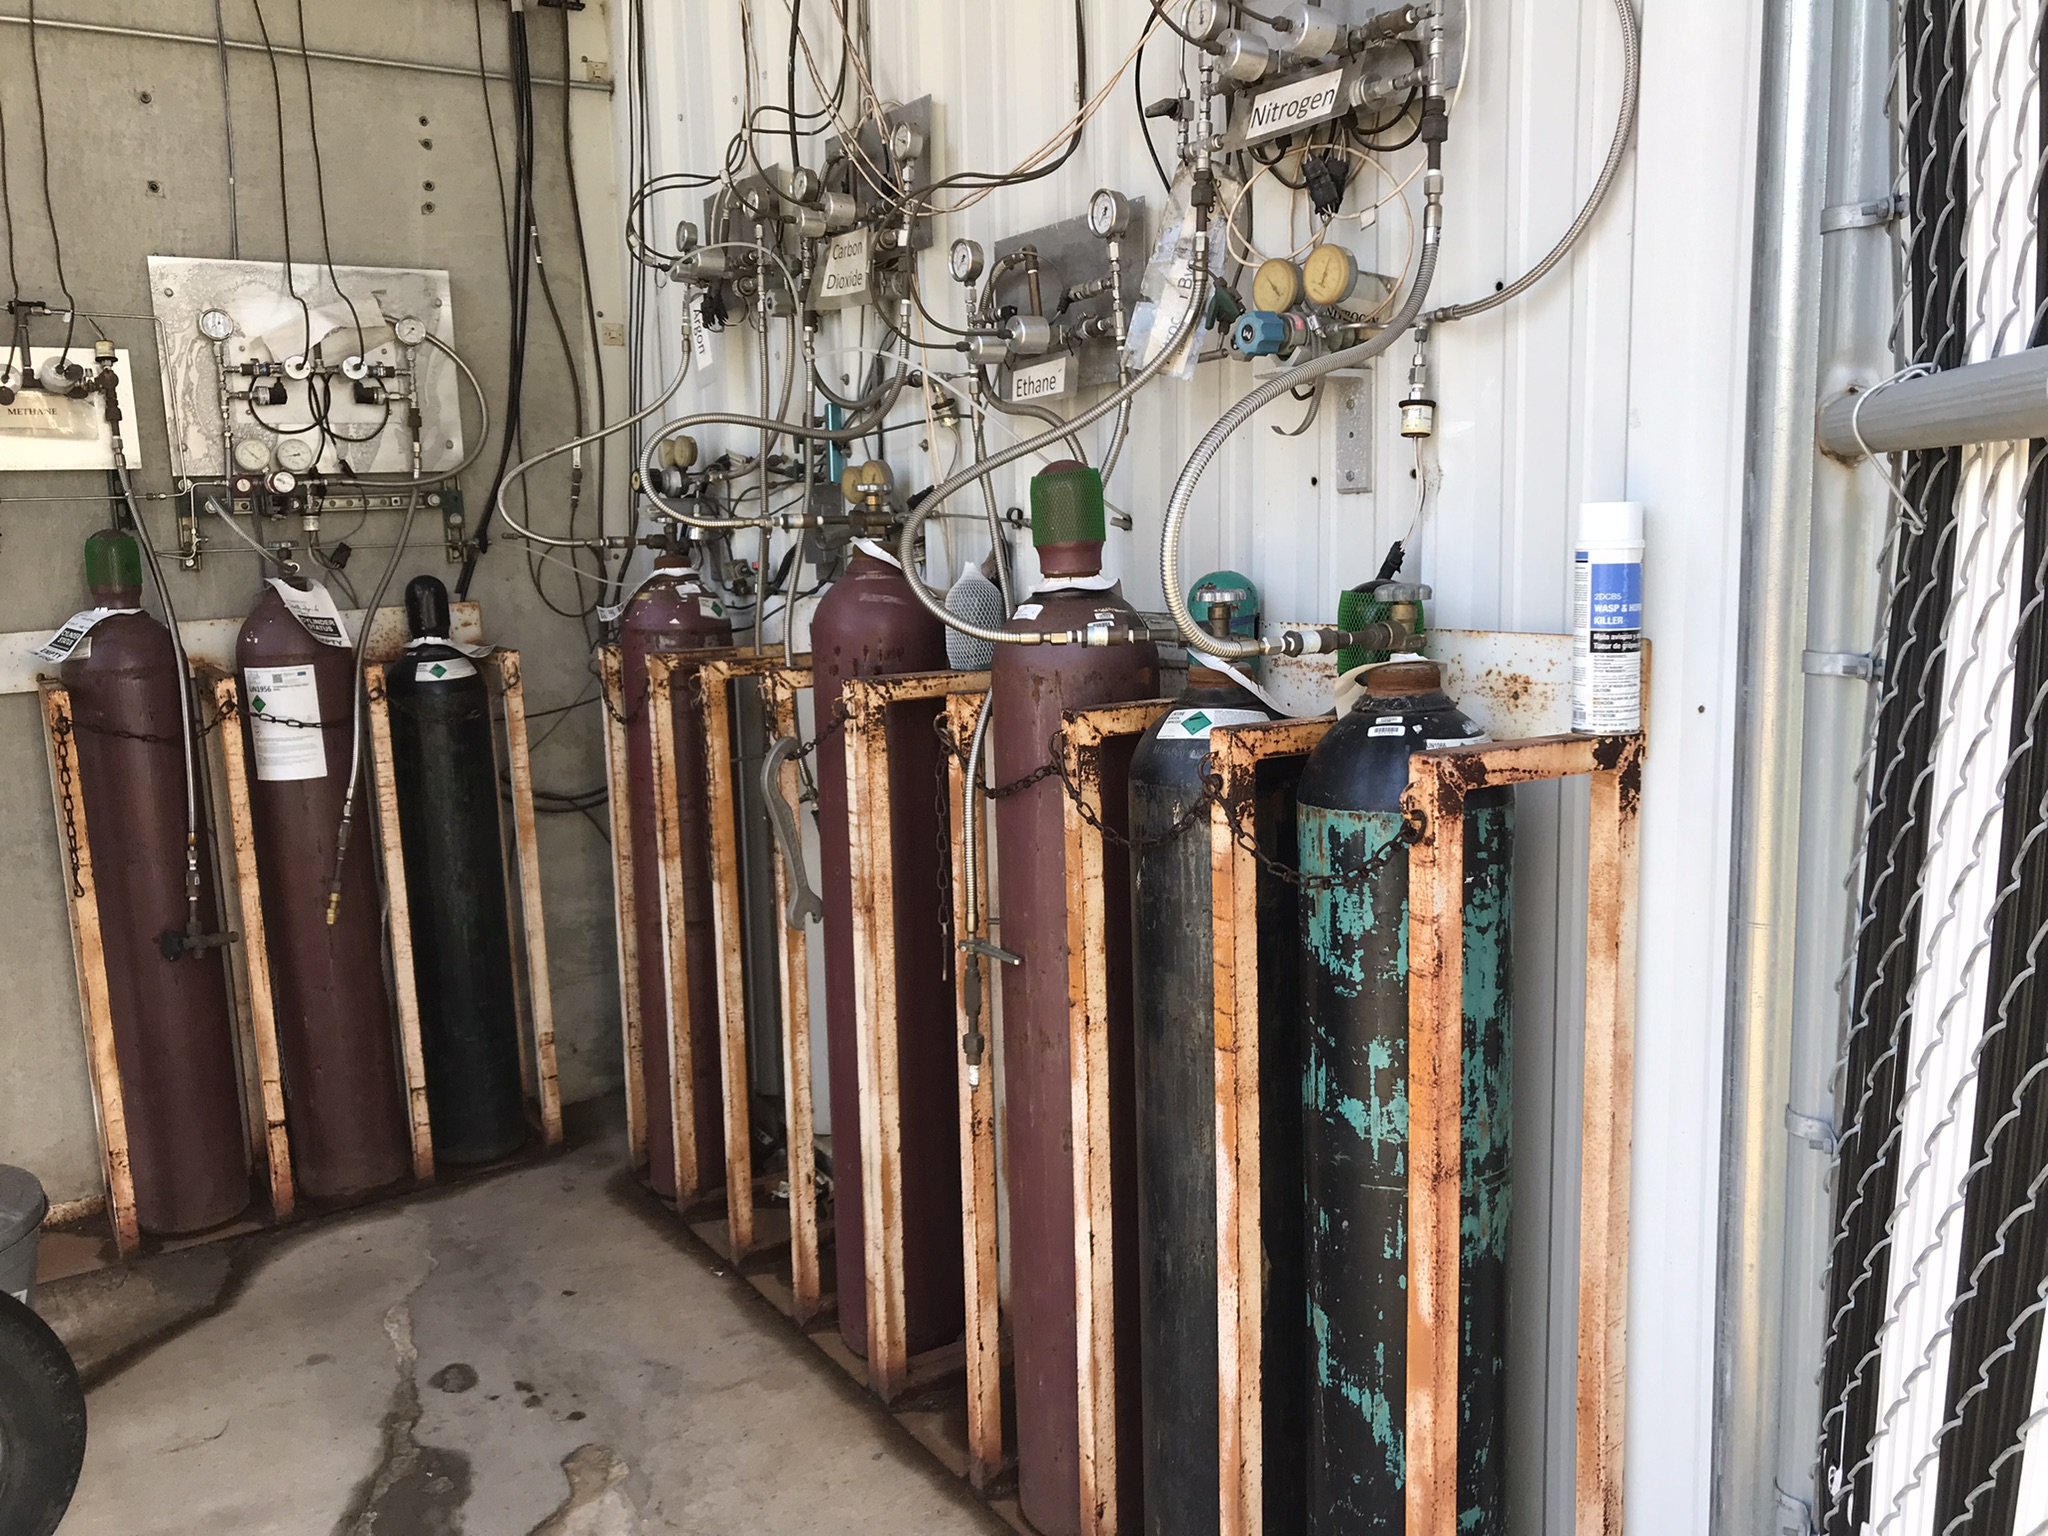
\includegraphics[angle=0,width=0.46\textwidth,clip]{OldGasSystemBottles.JPEG}
\caption{A photograph of the old gas system shed - gas racks and the manifolds. The right most two bottles (black color) are industrial nitrogen and are used for the bottle switchover.}
\label{fig:BottleOS}
\end{center}
\end{figure}
 For each gas type, two cylinders can be connected to a manifold at any point in time, one would be
 in use and another would be in the stand-by mode (connected to the manifold, but valved off).
 The switching between the bottles is electronically controlled by digital pressure sensors and
 a pneumatic switchover system that uses industrial nitrogen bottles (the two gas bottles on the rightmost side in Fig~\ref{fig:BottleOS}).
 This industrial N$_2$ is only used for controlling the pneumatic valve, it doesn't get mixed with
 the UHP gas that is used in the GEM detectors. A picture of the old gas system is shown in Fig.~\ref{fig:BottleOS}.
 This picture shows that the left-hand side Ar bottle, right-hand side CO$_2$, and two industrial nitrogen bottles (on the right side) are currently connected to the gas system. 

\begin{figure}[h!]
\begin{center}
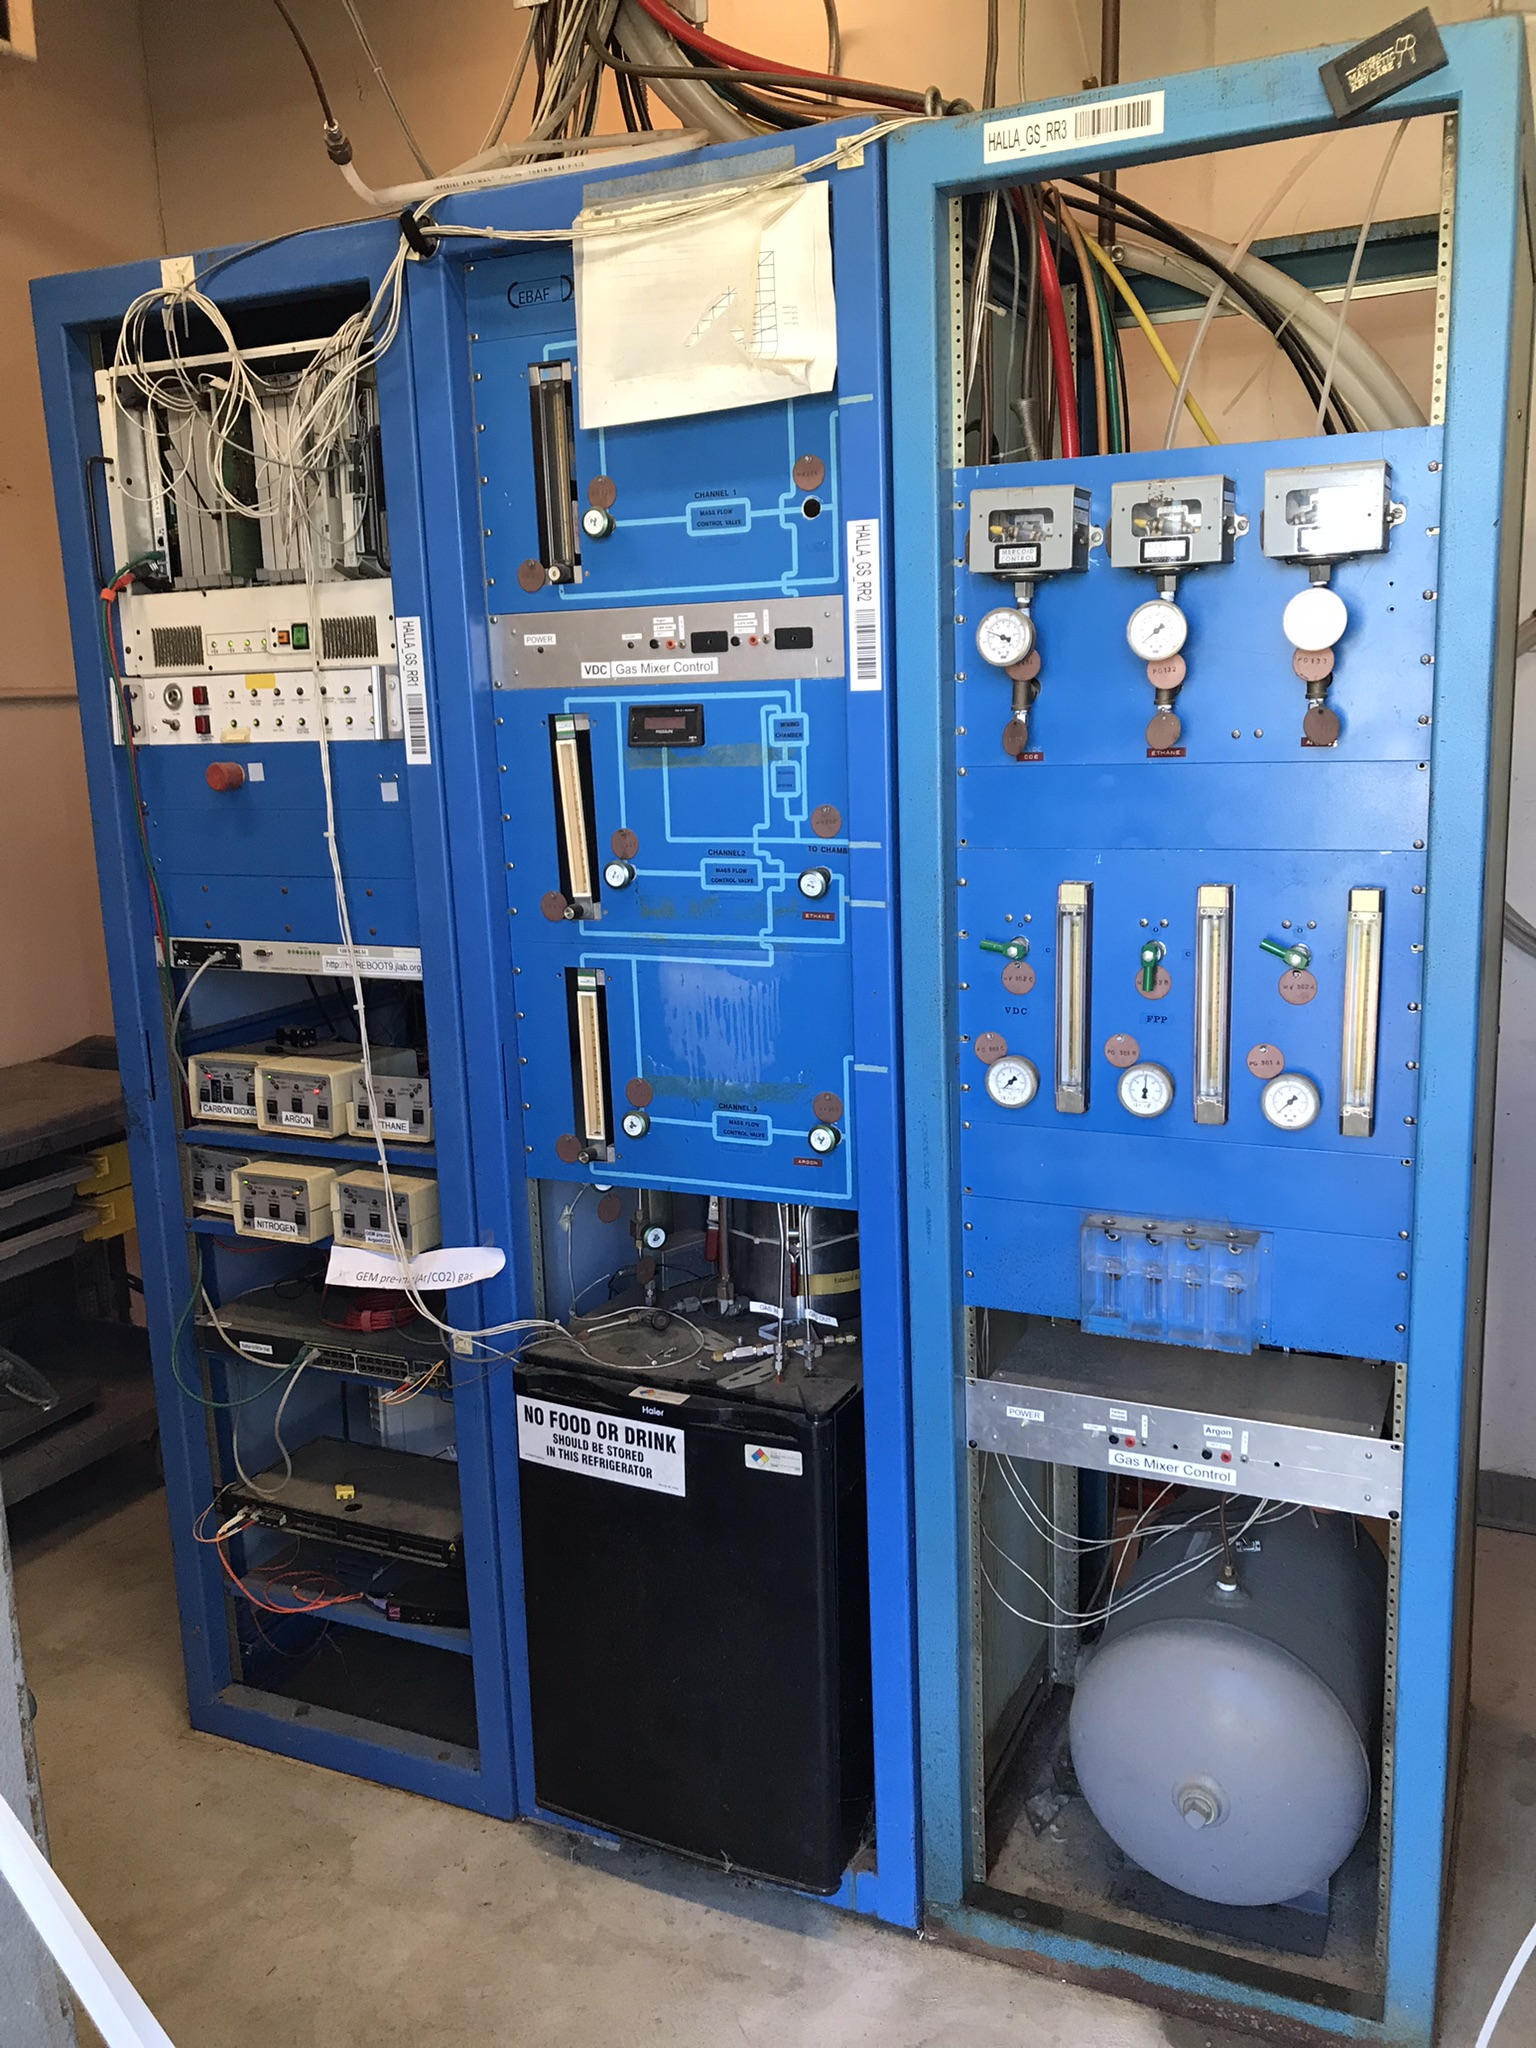
\includegraphics[angle=0,width=0.5\textwidth,clip]{OldGasSystemElectronics.JPEG}
\caption{A photograph of electronics racks. It contains the bottle-switching electronics (for the old gas system), and also for slow-controls. The mixing buffer tank for the old system is on the right bottom side of the rack.}
\label{fig:ElectronicsOS}
\end{center}
\end{figure}
The controlling electronics and the mixing unit are stationed in the rightmost room of 101A (on the right side of the Hall A truck ramp).
 A picture of the controlling electronics and the buffer gas tank (where the mixed gas is 
stored temporarily before sending into the hall) is shown in Fig.~\ref{fig:ElectronicsOS}.
 A close-up look of the controlling electronics for the old system is shown in Fig.~\ref{fig:ZoomedElecOS}.
\begin{figure}[h!]
\begin{center}
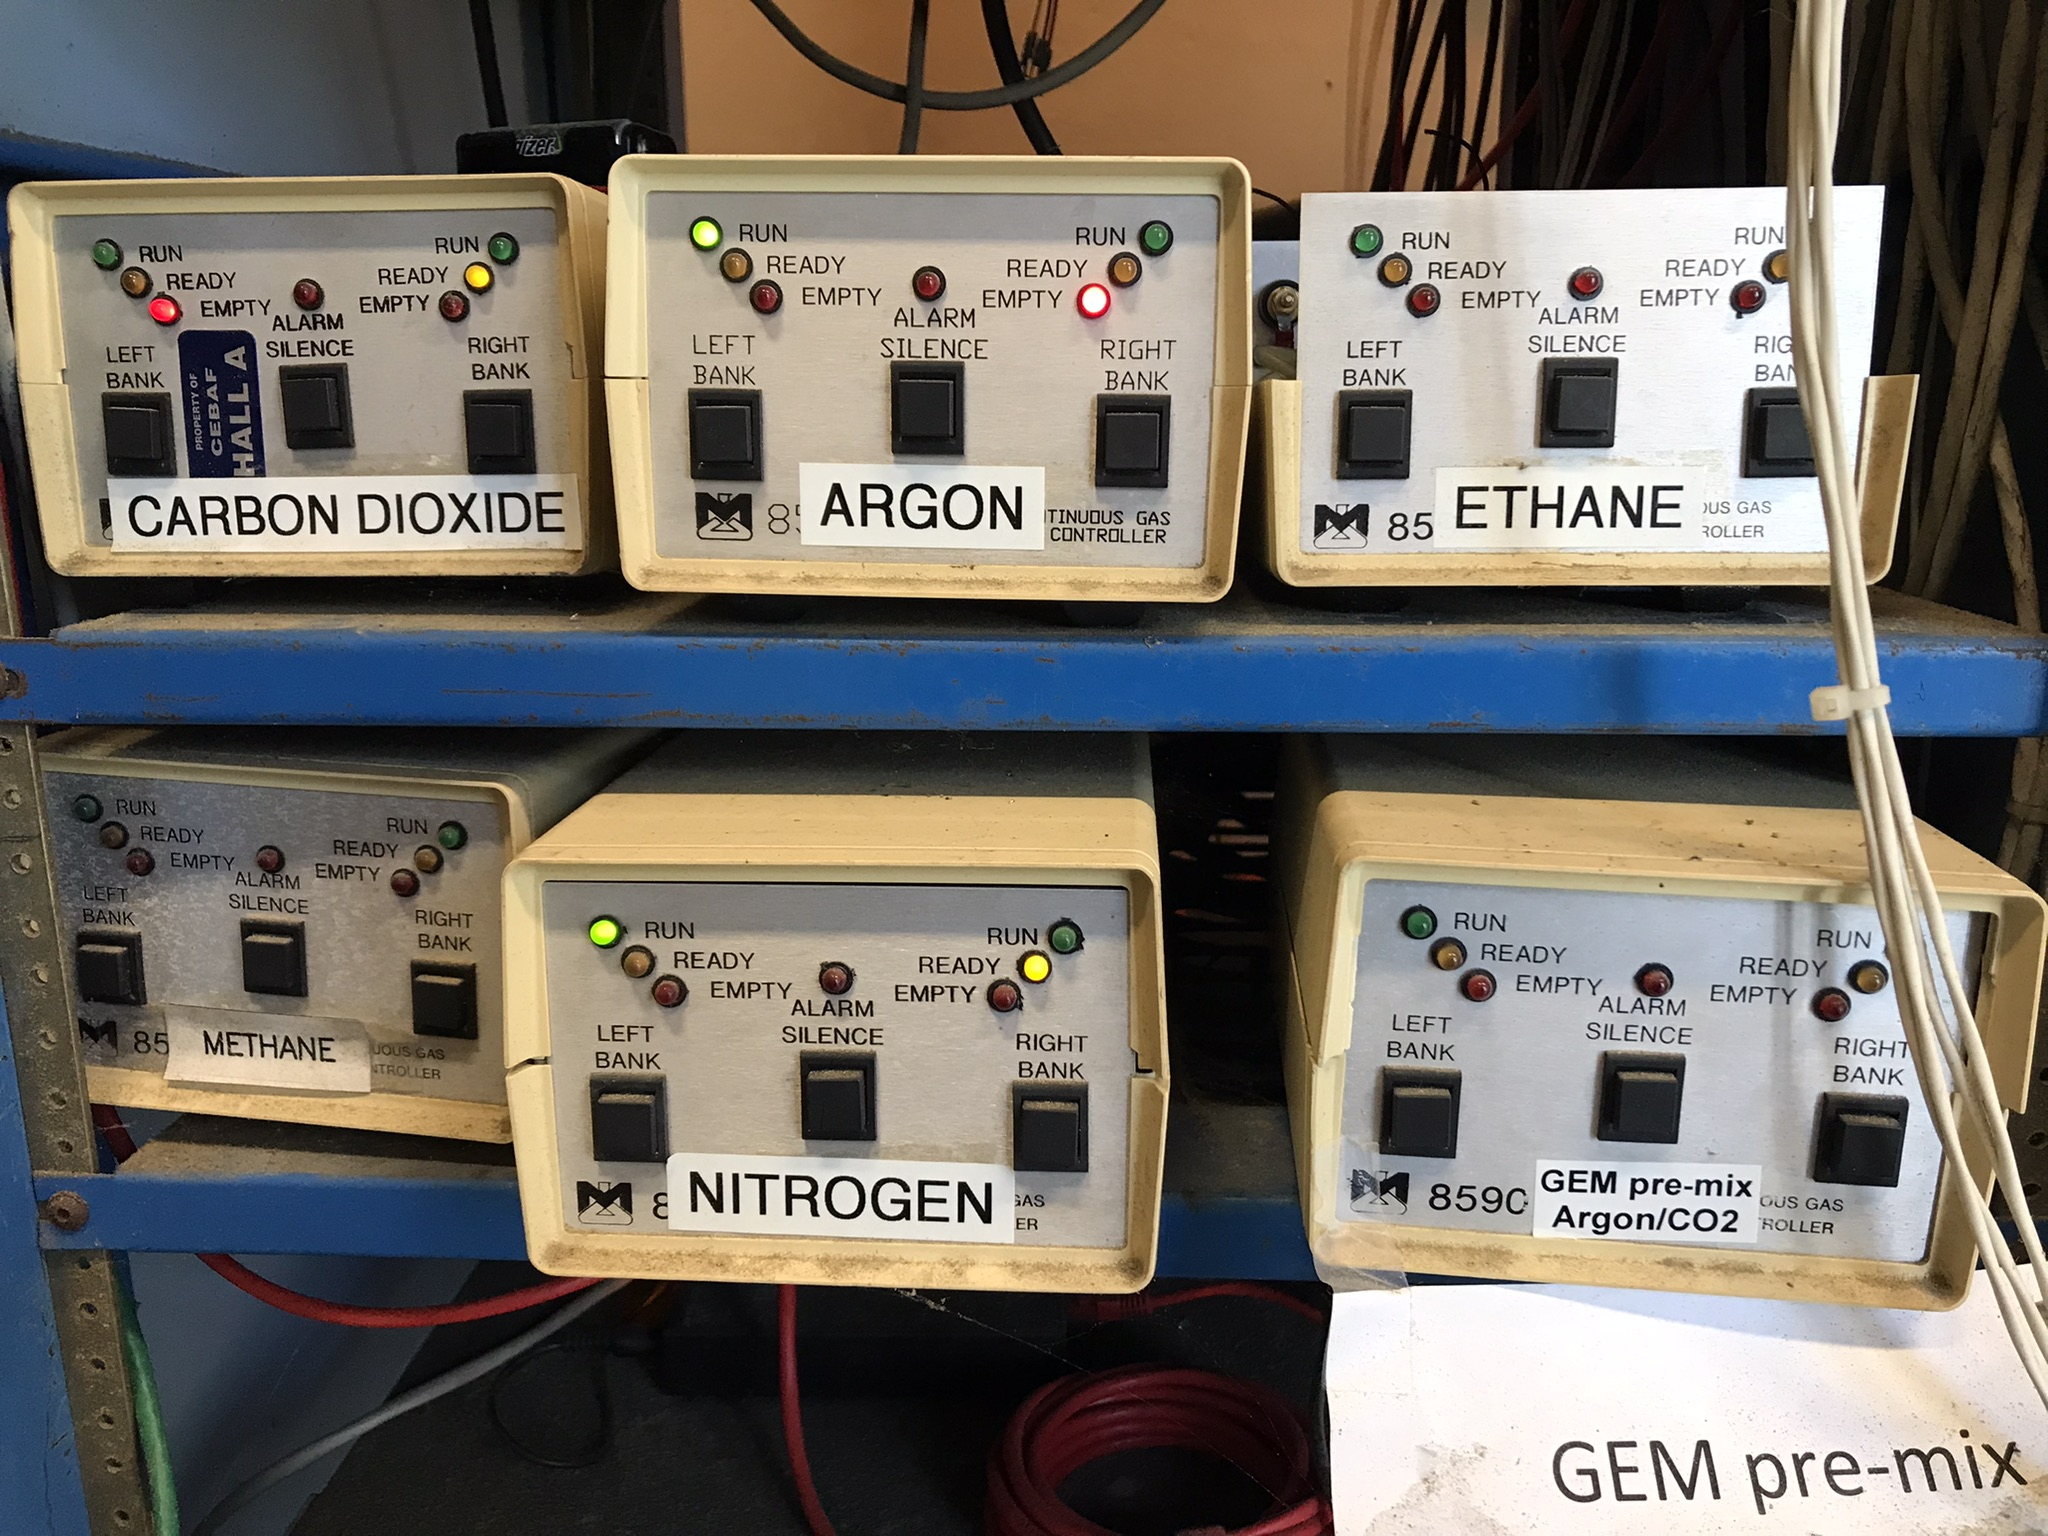
\includegraphics[angle=0,width=0.5\textwidth,clip]{OldGasSystemElectronicsZoomed.JPEG}
\caption{A close-up look at the bottle-switching electronics for the old gas system. The LED lights represent the status (RUN, READY, EMPTY) of the cylinders that are shown in Fig.~\ref{fig:BottleOS}. As mentioned earlier the methane and ethane system are not in use currently.} 
\label{fig:ZoomedElecOS}
\end{center}
\end{figure}

Two mass-flow controllers (MFCs) are used to get the desired gas mixing ratio.
 These MFCs are controlled by a custom-made electronics unit and one can change
 the ratio by setting the voltages via two potentiometer settings.
 For the old system, the MFCs are on the back side of the rightmost rack in Fig.~\ref{fig:ElectronicsOS},
 and the custom electronics box is on the same rack --just above the buffer tank.
 A photograph of the MFCs for the old system is shown in Fig.~\ref{fig:OldSystemMFC}.

\begin{figure}[h!]
\begin{center}
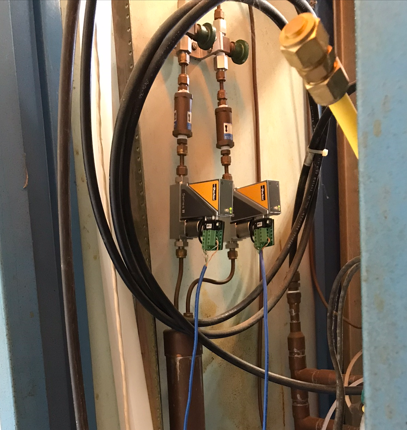
\includegraphics[angle=0,width=0.5\textwidth,clip]{OldSystemMFC.PNG}
\caption{The mass-flow controllers (MFCs) for the old system are on the rear side of the rightmost rack.} 
\label{fig:OldSystemMFC}
\end{center}
\end{figure}

The individual bottle (Ar, CO$_2$, and N$_2$) pressure, the pressure on the gas common line in the manifold
 (after the check-valve for each bottle for each type of gas), and set- and readback-values
 of the MFCs are archived through the EPICS interface. The gas-mixig ratio (Ar in CO$_2$) is
 also archived and shown in Fig.~\ref{fig:StripChartOldSystem}. 
\begin{figure}[h!]
\begin{center}
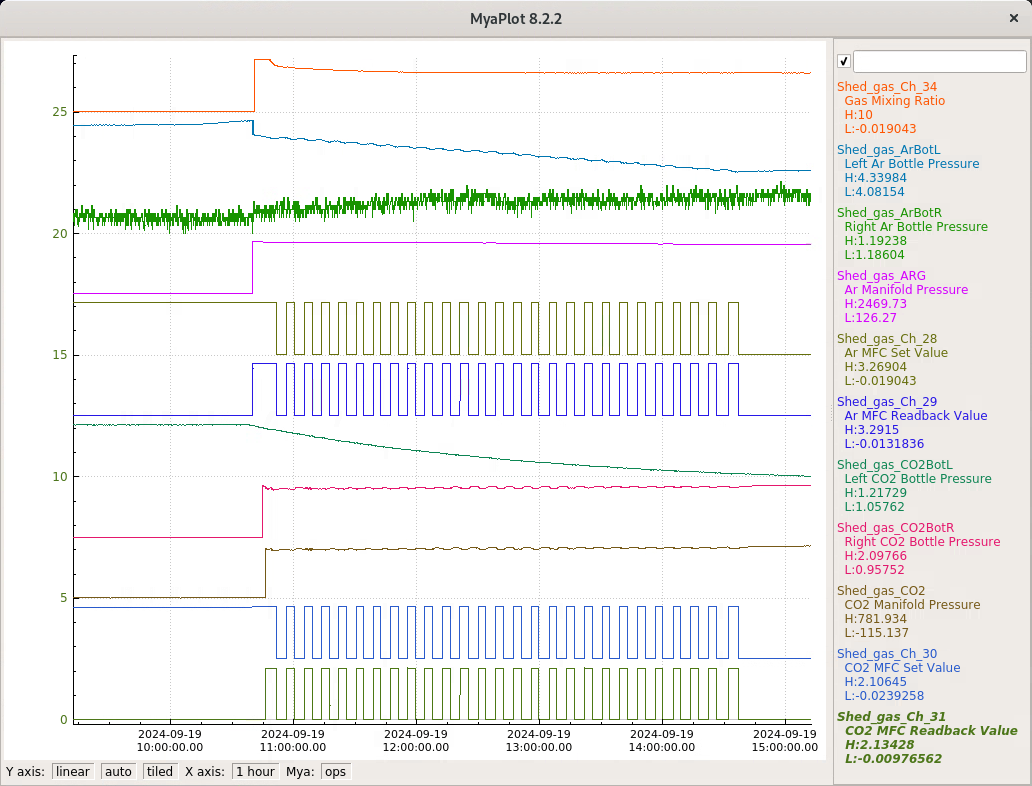
\includegraphics[angle=0,width=0.7\textwidth,clip]{OldSystemStripCharts.PNG}
\caption{The EPICS variables for the Ar-CO2 bottle pressures, set- and readback-values of the MFCs, and the gas mixing ratio for the old gas system.} 
\label{fig:StripChartOldSystem}
\end{center}
\end{figure}

\begin{figure}[h!]
\begin{center}
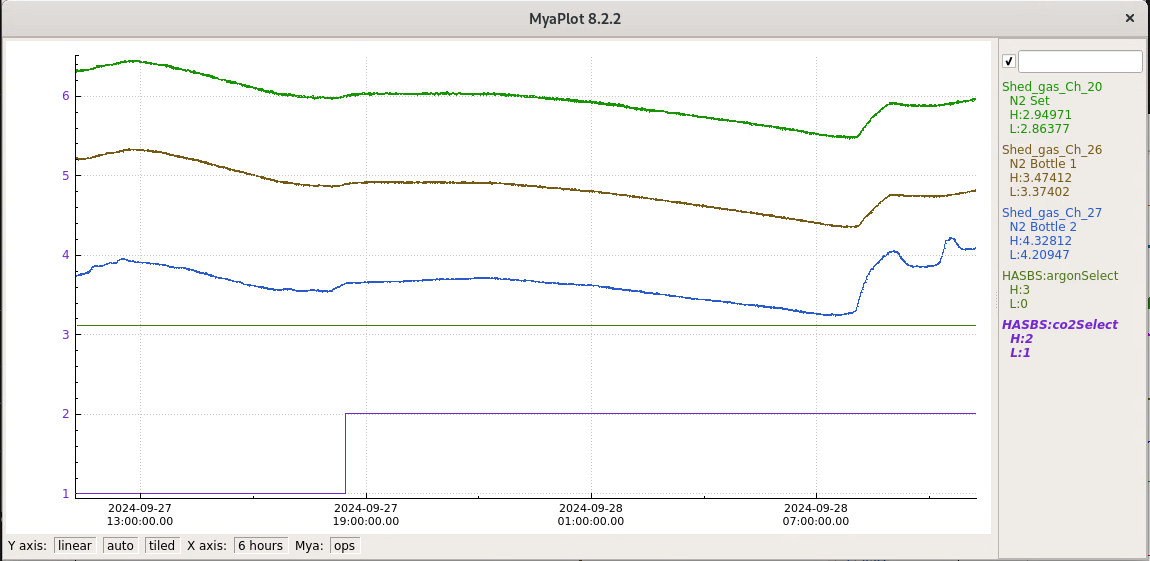
\includegraphics[angle=0,width=0.7\textwidth,clip]{SwitchingN2Bottle.PNG}
\caption{The EPICS variables for the Nitrogen bottle pressures.} 
\label{fig:NitrogenStripChart}
\end{center}
\end{figure}
To get the percentage mixing ratio, the PV Shed\_gas\_Ch\_34 needs to be multiplied by 10.
 From Fig.~\ref{fig:StripChartOldSystem}, one can see that the right side Ar and both CO$_2$ bottles
 were empty at 10 am on 19th Sept. Around 10:45 am, the right side CO$_2$ bottle was connected to the
 system and started filling the buffer tank until around 4:30 pm (at this point, the gas usage was stopped).
 The MFC set- and readback-values can be nicely seen in this figure.
 A similar figure for the nitrogen bottle pressures is shown in Fig.~\ref{fig:NitrogenStripChart}. 
 A manual on how to open the Jlab archiver (jmenu) and access the slow control variables for the Hall A gas system is in the halog entry https://logbooks.jlab.org/entry/4318342.

\section{The New Gas System}

  A new gas system (henceforth mentioned as the new gas system) was designed to meet the large gas volume requirement for the SBS GEM detectors 
and stationed on the left-hand side of the hall A truck ramp. In this system at any point in time,
 seven Ar bottles and three CO$_2$ bottles can be connected. The individual bottle pressures are monitored by 
digital pressure sensors and are archived using a Raspberry Pi (rpi).
\begin{figure}[h!]
\begin{center}
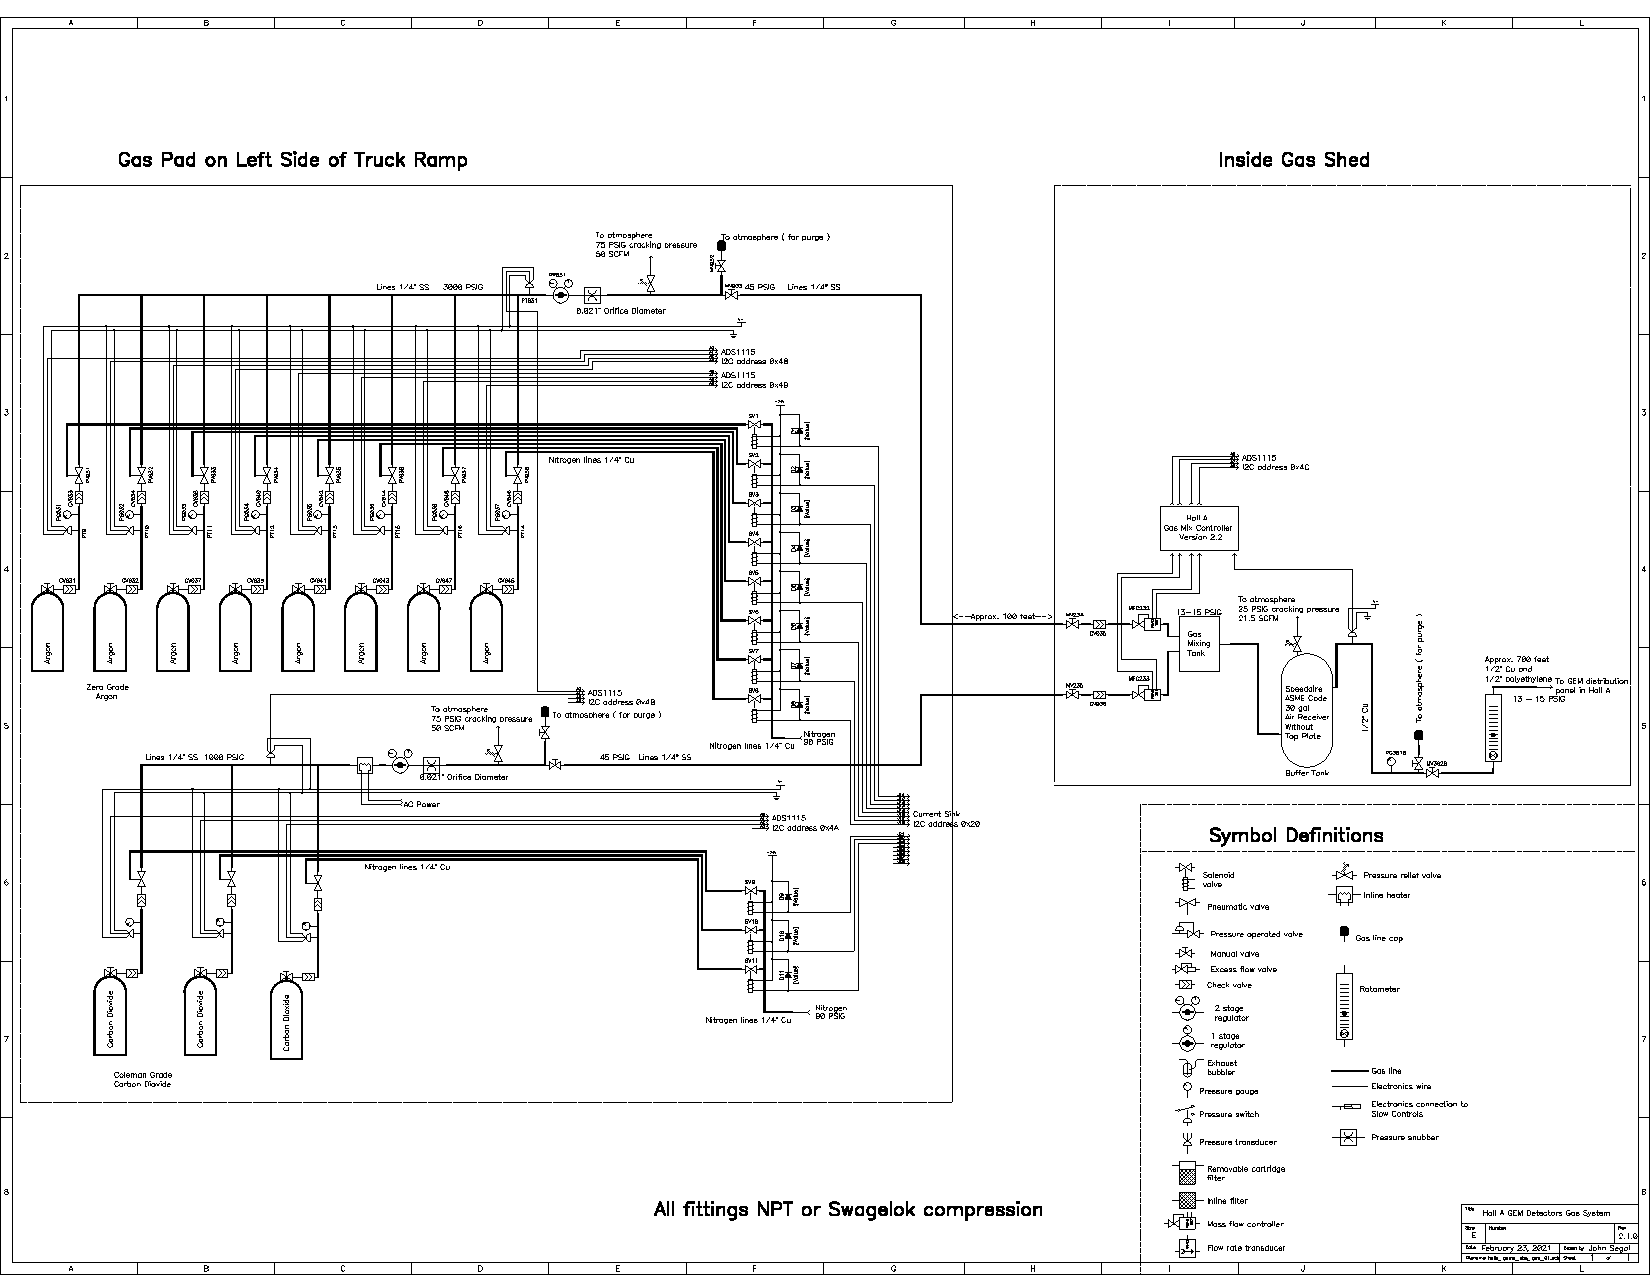
\includegraphics[angle=0,width=0.9\textwidth,clip]{gas_system_new.pdf}
\caption{Schematic of the new gas system. This system is modified to accommodate boil-off nitrogen gas from a liquid nitron dewar.}
\label{fig:NewSystemSchematic}
\end{center}
\end{figure}
 The automatic bottle switchover is done by activating pneumatic valves using the industrial nitrogen bottles
 mentioned in the old gas system.
 The two gas lines (one for Ar and another for CO$_2$,  hereafter mentioned as transfer lines) go to the gas hut on the right side of the truck ramp where they are mixed with the desired ratio and 
stored in a buffer tank before sending the gas to the hall.
 The pressure of the two gas lines is regulated to 45 psig as required by the MFCs. 
As a safety precaution, a 75 psig release valve is installed in the lines that go to the gas hut.
 A schematic of the new gas system is shown in Fig.~\ref{fig:NewSystemSchematic}. A picture of the new gas shed is shown in Fig.~\ref{fig:NewSystemBottles}.
\begin{figure}[h!]
\begin{center}
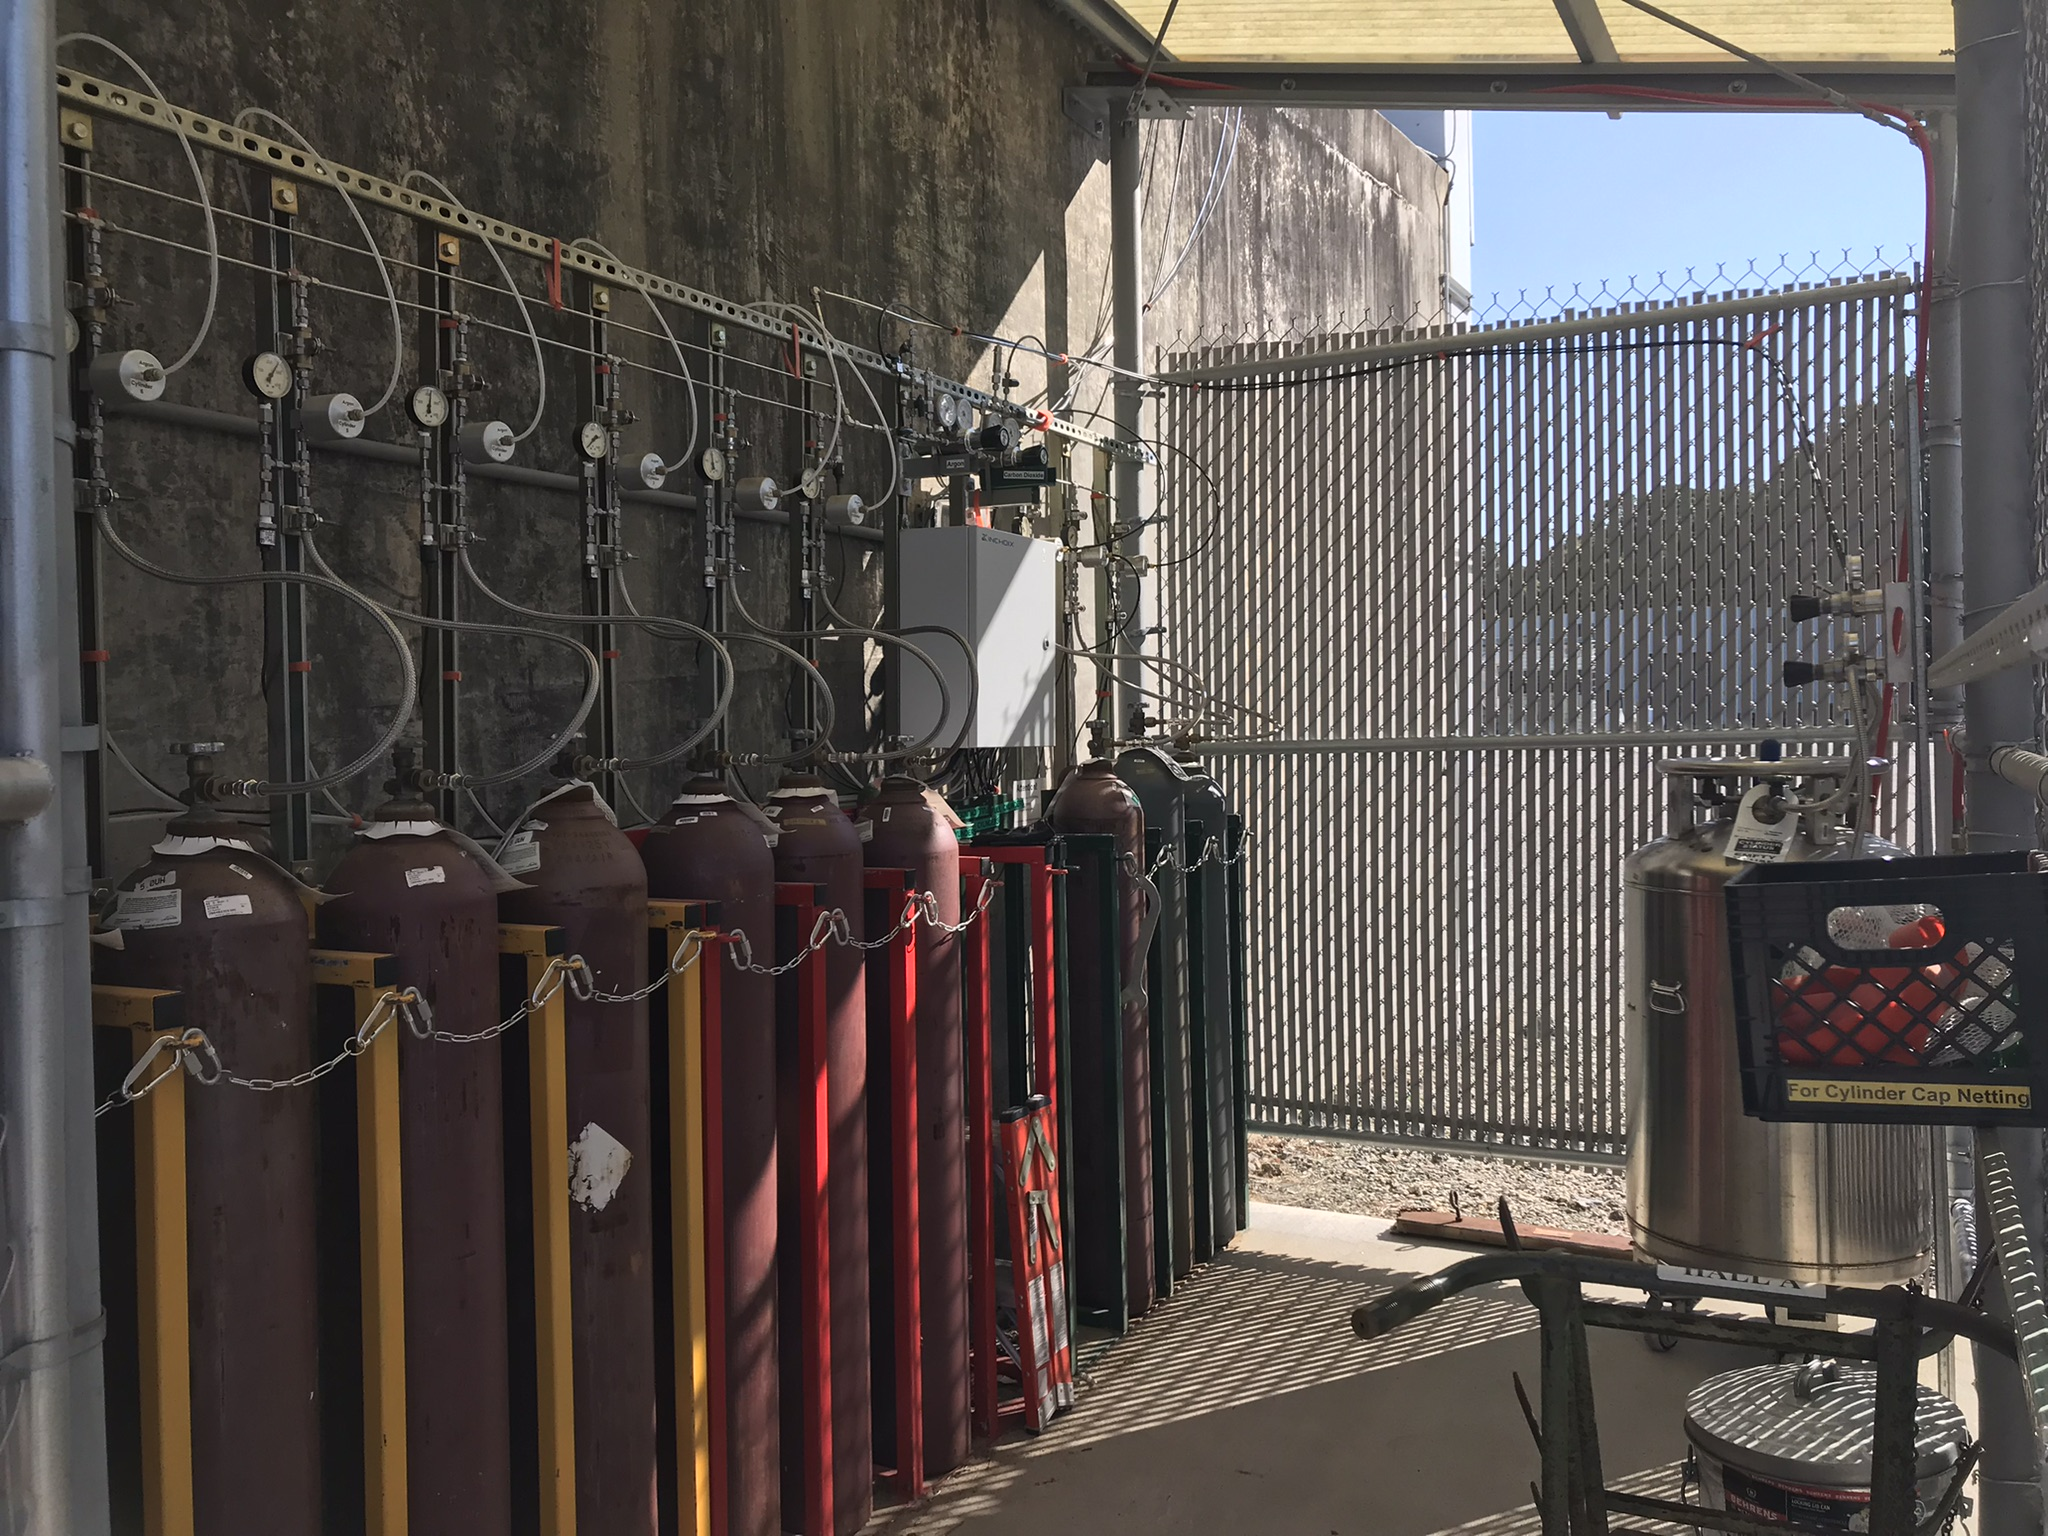
\includegraphics[angle=0,width=0.5\textwidth,clip]{NewGasSystemBottles.JPEG}
\caption{Gas racks and manifolds for the new gas system bottles on the right side of the truck ramp. The dewar and its regulator are on the right side of this picture.}
\label{fig:NewSystemBottles}
\end{center}
\end{figure}

A close-up picture of the regulator section of the new gas system is shown in Fig.~\ref{fig:NewSystemMod}. 
The new gas system is modified to accommodate nitrogen gas from a liquid nitrogen dewar.
 Two dewars can be connected to the regulator placed in the new gas hut 
(see dewar on the right-side in Fig.~\ref{fig:NewSystemBottles}). Care should be taken to connect the 'gas' port of the dewar to the gas system.
 Two gas lines from this regulator are brought to the other side of the shed
 where the Ar- and CO$_2$-regulators are situated (Fig.~\ref{fig:NewSystemMod}). Each of the two gas lines is connected
 to the low-pressure side of the Ar and CO$_2$ regulatoris of as shown in Fig.~\ref{fig:NewSystemMod} (the black poly tubes). In this way, both the transfer lines will
 bring boil-off N$_2$ to the gas hut where it can be used for both the old and the new gas systems
 (after a little modification which has not been done as we never used boil off nitriogen in the old system).
 This was done to avoid to transferring a dewar from the left side to
 the right side of the truck ramp where the old gas system's bottles are. 

\begin{figure}[h!]
\begin{center}
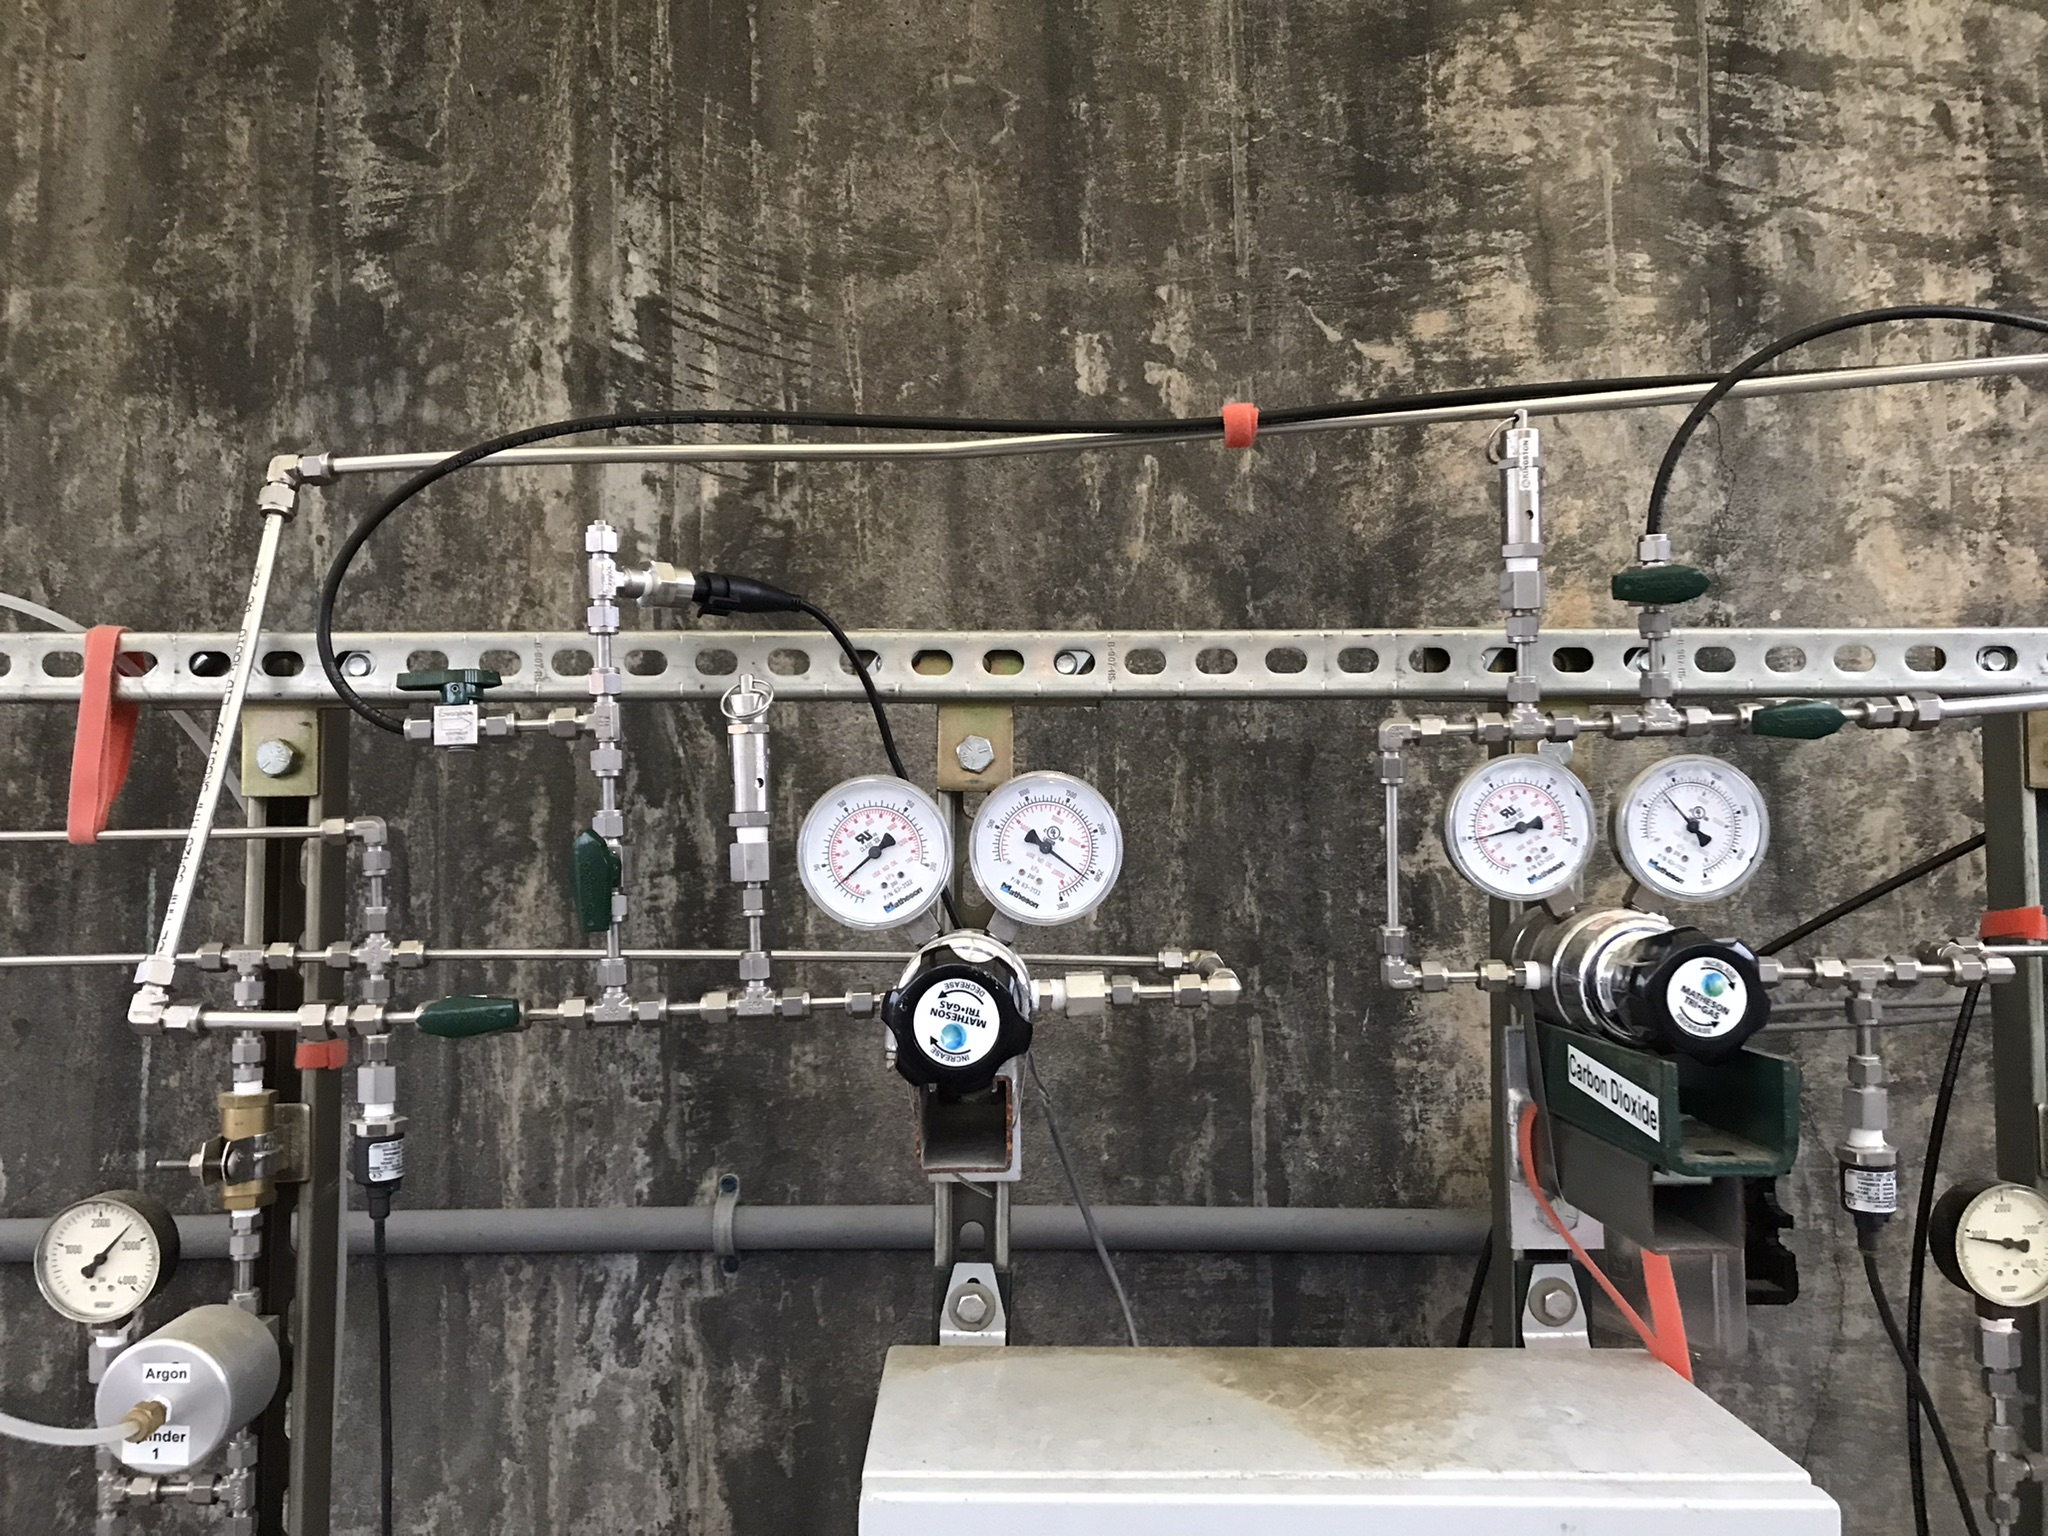
\includegraphics[angle=0,width=0.7\textwidth,clip]{NewGasSystemMod.JPEG}
\caption{A close-up look of the regulators of the new gas system. This system is modified to accommodate boil-off nitrogen gas from a liquid nitrogen dewar. The black tubes in this picture are from the dewar.}
\label{fig:NewSystemMod}
\end{center}
\end{figure}

The transfer lines from the new gas shed come to the gas hut where they are mixed and kept inside a 30 gal buffer
tank before sending the gas mixture to the hall with 15 psig pressure. The MFCs and their controlling electronics are
 shown in Fig.~\ref{fig:NewSystemMFC}. In the outlet of the buffer tank, the binary gas analyzer (BGA)
 is connected to measure and monitor the gas mixing ratio. One should select the gas types 
from the BGA window to get the correct gas mixing ratio. Sometimes, the users request to cross-calibrate the BGAs
using a premix bottle from the vendor. The premix bottle can be directly connected to the BGA via a two-stage regulator.
 After flowing through some gas from the premix bottles, note the reported mixing ratio by the BGA. The reported number should be close to the premix ratio of the bottle if the proper gas types are selected in the BGA. An elog entry about this process and its result can be found in the halog entry 4293968.   

\begin{figure}[h!]
\begin{center}
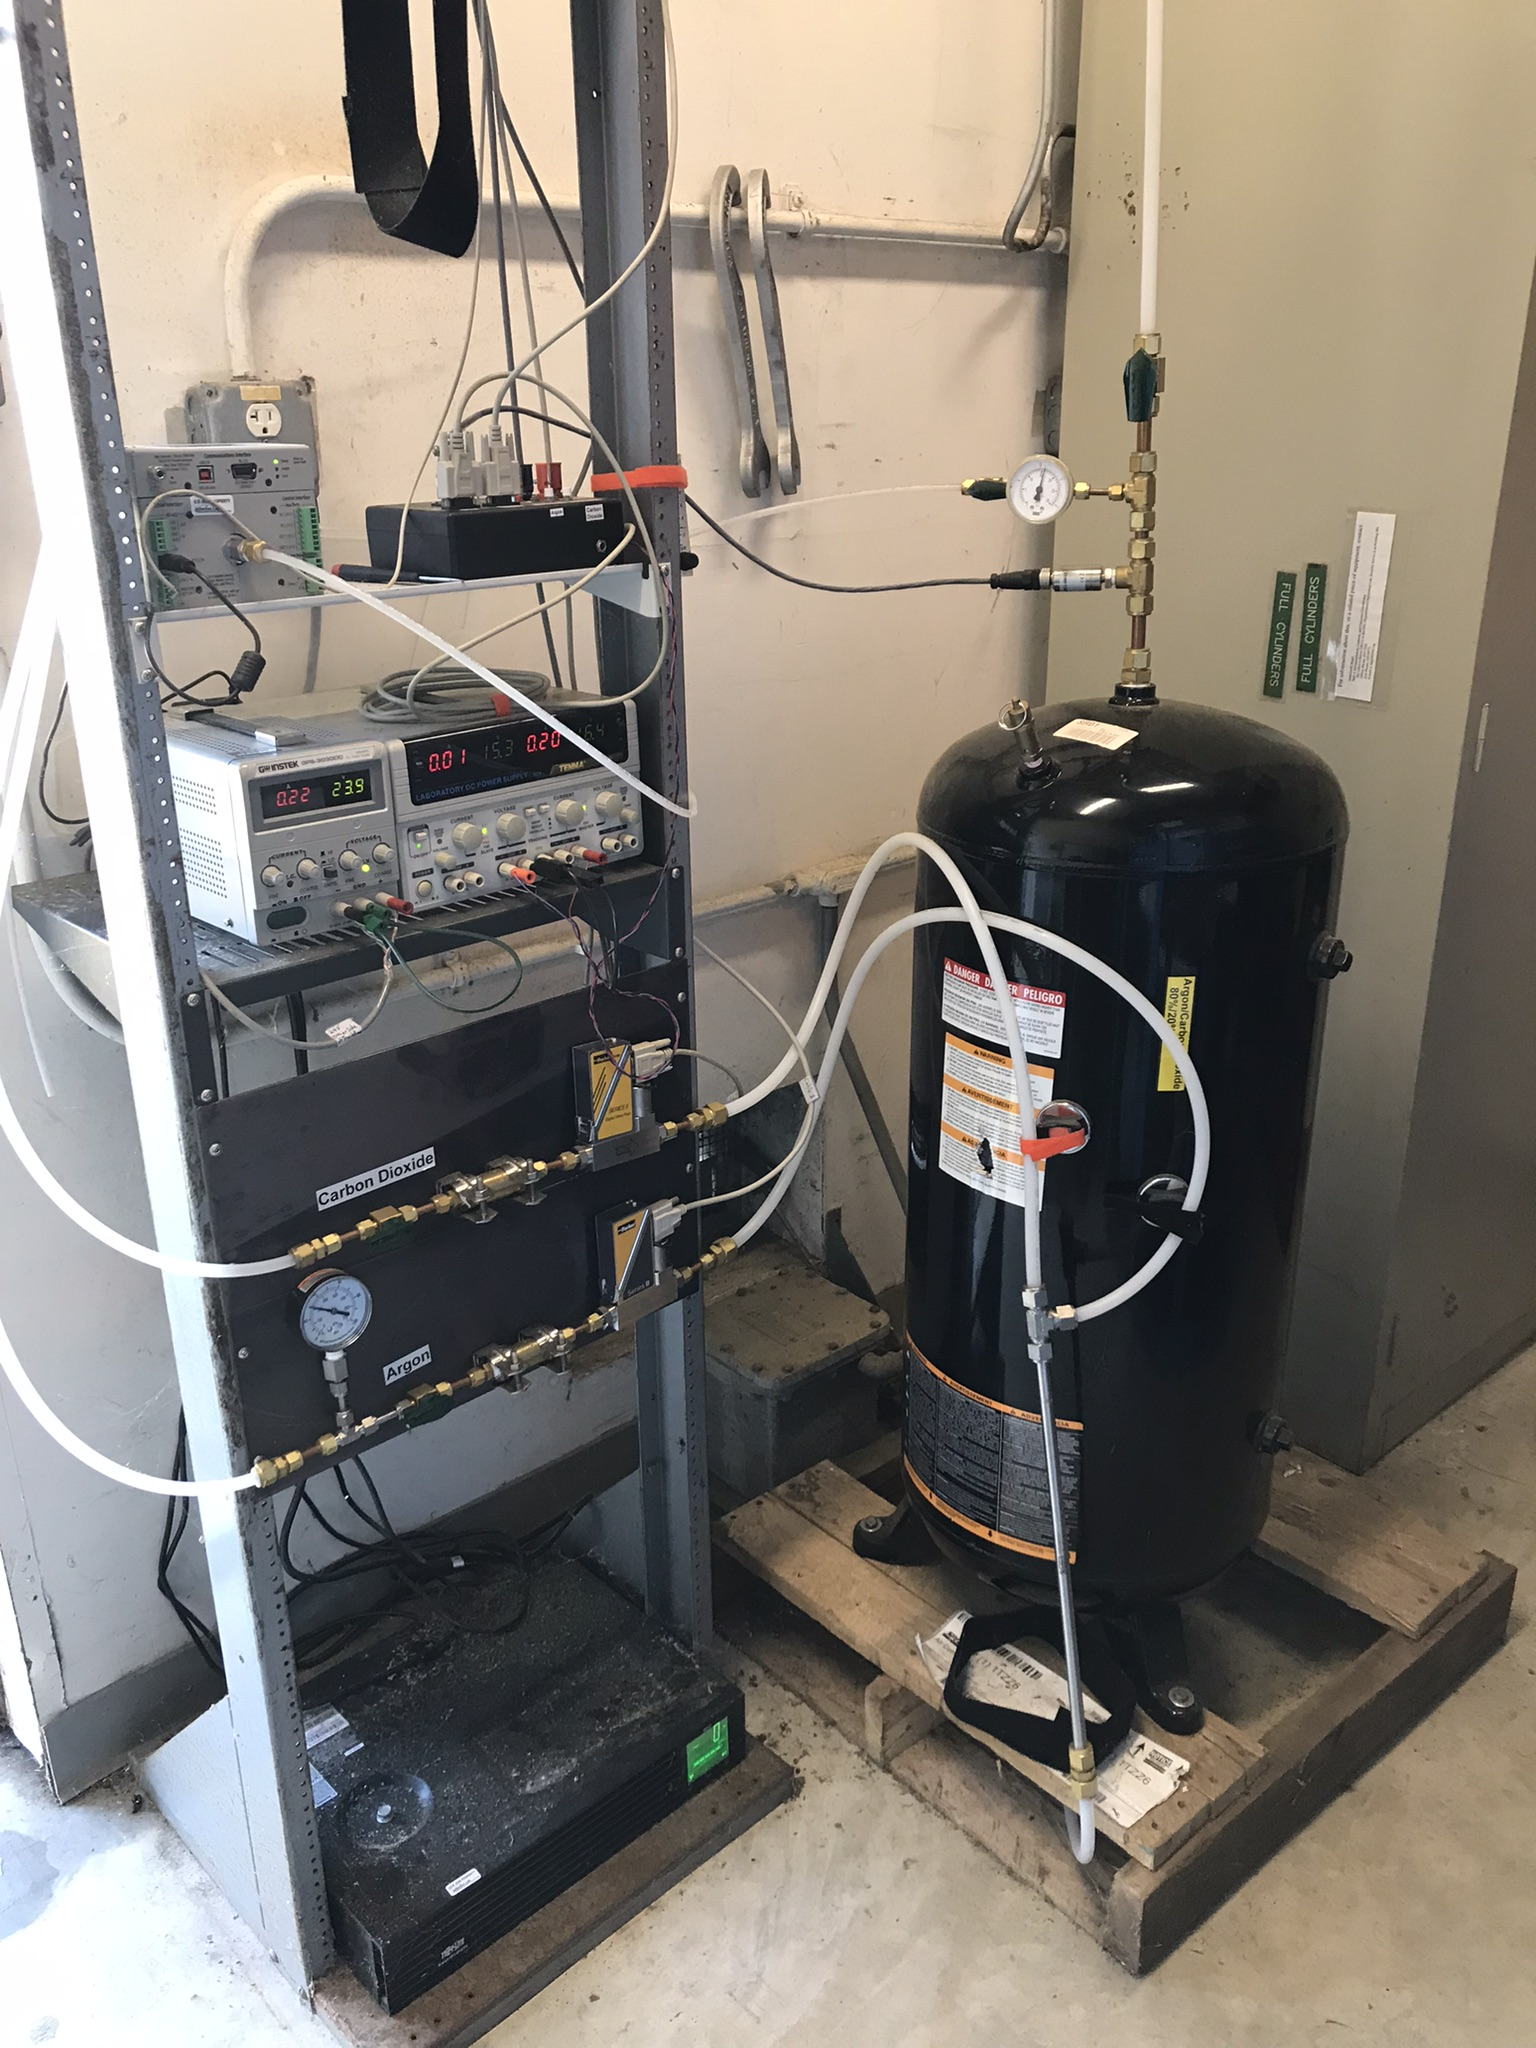
\includegraphics[angle=0,width=0.4\textwidth,clip]{NewGasSystemMFC.JPEG}
\caption{The Mass-Flow Controllers and buffer tank of the new gas system.}
\label{fig:NewSystemMFC}
\end{center}
\end{figure}

Like the old gas syetem, the individual pressure of the botlles, the gas mixing ratio are archived using
 the EPICS interface. The strip charts for the new gas systems are shown in 
Fig.~\ref{fig:NewSystemStripChart1} and Fig.~\ref{fig:NewSystemStripChart2}. Please look at the halog entry 4318342 to know more about the slow control variables.

\begin{figure}[h!]
\begin{center}
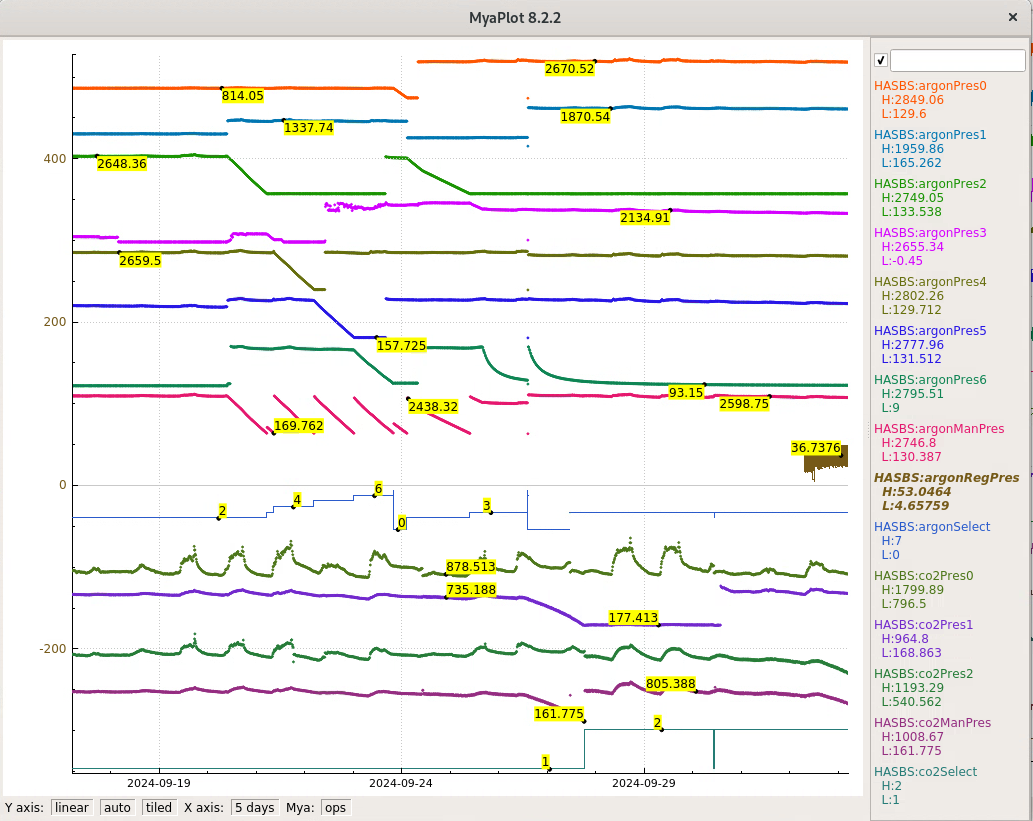
\includegraphics[angle=0,width=0.8\textwidth,clip]{NewSystemIndividualBottleMonitor.PNG}
\caption{Slow control variables of individual bottle pressures of the new gas system}
\label{fig:NewSystemStripChart1}
\end{center}
\end{figure}

\begin{figure}[h!]
\begin{center}
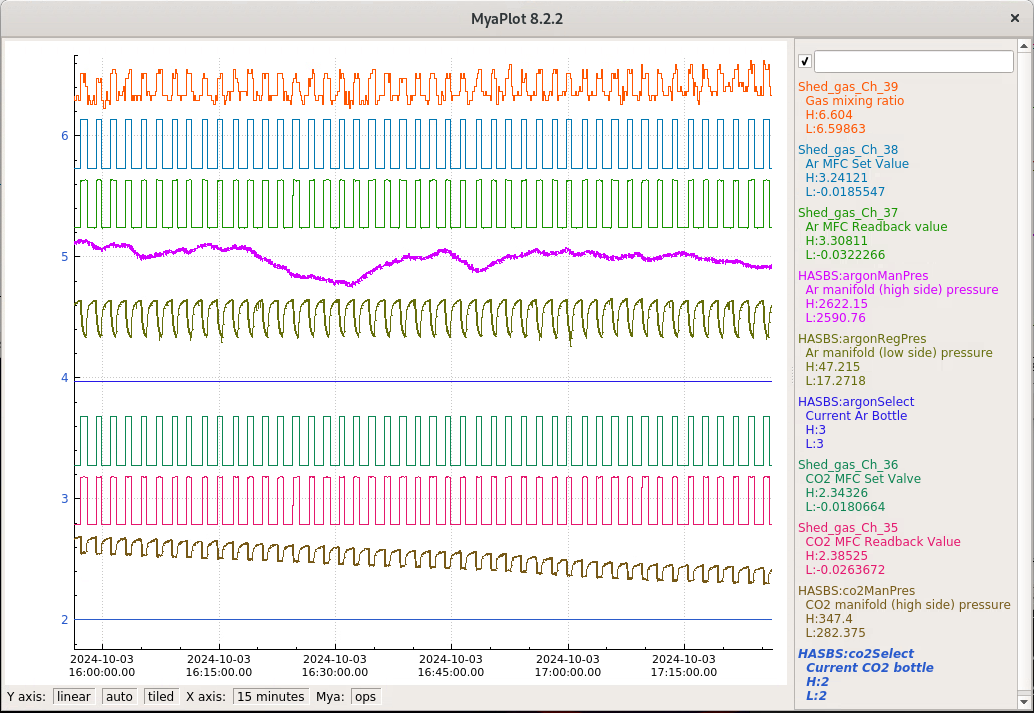
\includegraphics[angle=0,width=0.8\textwidth,clip]{NewSystemMixingRatio.PNG}
\caption{The slow control variables of the gas mixing ratio, set- and readback-values of the MFCs of the new gas system.}
\label{fig:NewSystemStripChart2}
\end{center}
\end{figure}

\section{Gas Storage racks}
The gas storage rack is on the left-hand side of the hall A truck ramp -just outside of new gas system's shed.
 There are multiple racks where a total of 66 bottles can be stored. Some of the racks are designated for the empty bottles using magnetic stickers.

\section{Gas Delivery into Hall A}
Between the gas shed and the two Hall-A shield houses are several gas
line runs of about 700 feet in length through the truck ramp.
The two lines used for the GEM detectors go to the gas distribution manifolds in the Hall. The manifolds in the hall are currently located on the right side of the pivot area. The pressures in all of these lines is nominally 15 psig.

\section{How to change cylinder in the system}
\begin{itemize}
\item
 Look at the pressure gauge connected to the bottle that needs to be changed. If zero or below a preset value, then
 close the cylinder using the handwheel valve on the top of the cylinder.
\item Unscrew the CGA 580 (for Ar, N$_2$, or dewar) or CGA 320 (for CO$_2$) adapter slowly.
\item Put the gas cylinder cap, and make sure it is tightened properly.
\item Remove the securing chain of the gas rack and take the cylinder to the empty gas rack outside the new gas stand.
\item Bring a new cylinder, put it inside the gas rack, and ensure the securing chain is properly placed.
\item Open the gas cap and see if the adaptor plug is clean. If not, put a label on that cylinder and notify Donald Brown. Use a new cylinder.
\item If the adaptor plug is clean, connect the adaptor and tighten it with a snug - no need to have a super tight. But a hand tight is not good.
\item Slowly open the valve. Make sure there are no leaks (if you don't hear any hissing sound and don't feel any flow when you put your hand near the connection, that is enough).
\item Check the pressure on the gauge connected to the new bottle that has just been replaced. If a new bottle is connected it should show $\sim$2700 psig for Ar, $\sim$2200 psig for N$_2$, and $\sim$1000 psig for CO$_2$.
\end{itemize}


\section{How to change from cylinder to dewar}
\label{bottlechange}
This is required when the GEM detectors will not be in use and need to be purged.
 The boil of nitrogen option is cheaper than using the UHP nitrogen bottles. 
Also, for the full load of the SBS GEM systems, a dewar can run for two weeks, 
whereas a 304 cf nitrogen bottle can run for $\sim$~20 hours. 
Hence, we use the boil off nitrogen gas from the dewar. Typically in a dewar, there are three ports - one for liquid, one for vent and another for gas usage. Make sure to use the gas port only.
In a freshly filled dewar, the gas pressure is not very high. 
So, one has to open the pressure-building valve to build pressure. 
It takes around 5-10 min and can be confirmed by ice formation on the top of the dewar
 or on the bottom side of the dewar. If the pressure-building valve is opened too much,
 the gas pressure will build up and the gas will go to the atomsphere through a saftey release valve.
So, some back-and-forth opening and closing of the pressure-building valve is required to attain an optimum
setting. The dewar system doesn't have a reliable option to monitor the amount of liquid left
 inside the dewar and it doesn't have an automatic switching option like the gas bottles. 
So, it would be wise to use a small fraction of CO$_2$ to along with N$_2$ from a dewar. 
This would avoid situation like when the dewar run out in the middle of odd hours and the chambers would not get any gas flow.
 If that happens, there would still be gas flowing through the chambers if a small fraction of CO$_2$ is mixed with the dewar N$_2$.
Here are the steps one needs to follow to flow boil-off nitrogen from a dewar instead of Ar/N$_2$. 
\begin{itemize}
\item Ensure the dewar is connected to the gas port.
\item Check the pressure on the dewar and on the regulator close to the dewar. 
If pressure if more than 45 psig, then the dewar is ready for use. Otherwise, try opening the pressure-building option to build pressure.
\item If the dewar has reached to the optimum pressure, then control the regulator to achievei 45 psig outlet pressure.
\item Stop flowing Ar by closing the Ar side regulator (in Fig.~\ref{fig:NewSystemMod}).
\item Open the ball-valve that is directly connected to the gas line coming from the dewar (in Fig.~\ref{fig:NewSystemMod}).   
\end{itemize}

If the above steps are followed, then the system will be using boil-off nitrogen from the dewar. One can
ensure this by checking the reported gas mixing ratio from the BGA. The ratio should change. Also, don't forget to change the gas type for BGA (from its LED screen).
\section{Steps to follow if the both nitrogen bottles for Switching bottles run out}
If both the nitrogen bottles used for activating the pneumatic valves run out, then just a simple replacement
of the bottles will not activate the bottle changeover. To initiate bottle changeover properly after both the bottles
run out, the following steps need to be followed.
\begin{itemize}
\item Follow the steps in \ref{bottlechange} and replace both the N$_2$ bottles with industrial N$_2$ bottles. If industrial N$_2$ is not available, then UHP N$_2$ or Ar can be used.
\item Slowly open the handwheel valve of both cylinders. This will make a hissing sound for some time as the empty lines will get filled with the gas.
\item While the above step is going on, open the ball valve (black color in Fig.~\ref{fig:BottleSwitching}) that is near the pressure gauge of the left side bottle.
\item Keep the ball valve open until the pressure readings on both N$_2$ pressure gauges read the same valve, and the hissing sound of filling lines stops.
\item Close the ball valve mentioned above.
\end{itemize}

If this is done properly, then the Ar/CO$_2$ bottle switching will happen properly for both the old and new gas systems.

\begin{figure}[h!]
\begin{center}
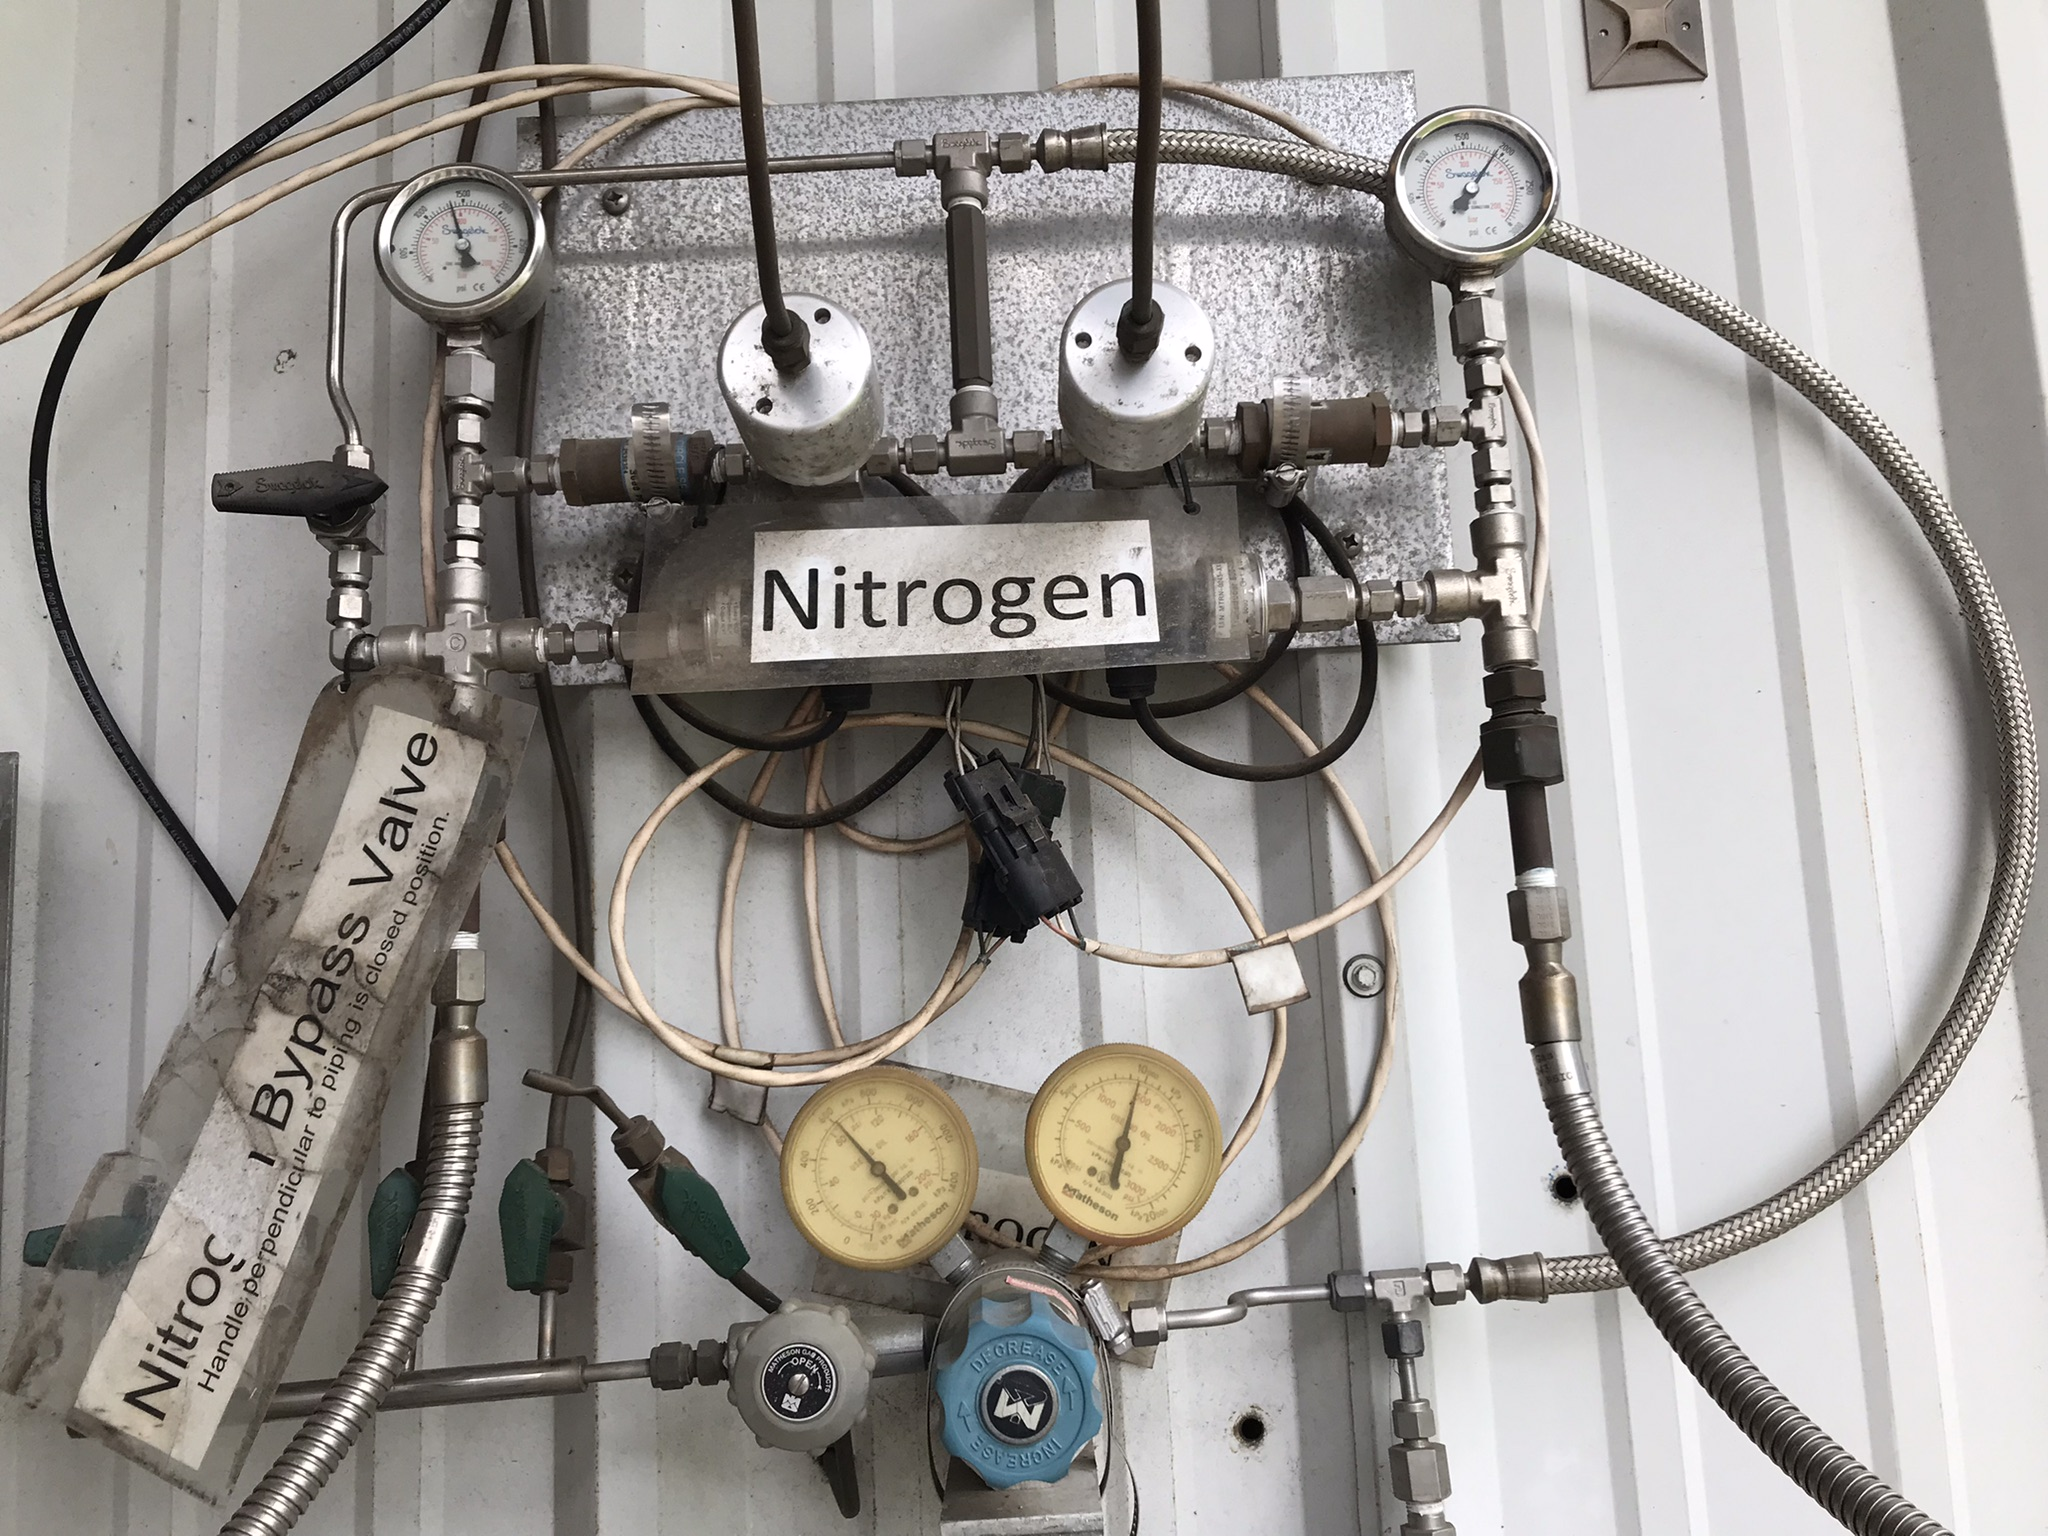
\includegraphics[angle=0,width=0.7\textwidth,clip]{SwitchingN2.JPEG}
\caption{The regulator for the nitrogen bottles used for bottle switching.}
\label{fig:BottleSwitching}
\end{center}
\end{figure}


\section{Control of MFCs and the buffer tank pressure}
Gas will be metered to each detector element through a flow meter.
To achieve a constant flow a constant
differential pressure must be maintained across it, so it is necessary
to provide a fairly constant supply pressure out of the mixing
station.  This comes only at a price, as the mass flow controllers
deliver a fixed {\it flow rate} regardless of pressure (within
practical limits).  If the detectors in Hall-A consume less gas than
the mixer supplies, the pressure in the supply lines will increase.
Similarly, if less gas is mixed than is consumed the pressure will
decrease.  To provide a usefully constant pressure of about 15 psig in
the supply line, a pressure switch/sensor is used in the
mixing station outlet.  The Pressure
Control Switch is set to open at 16 psig and close again at 14 psig
or below. As mentioned earlier, a custom-made electronics unit is used to control
these pressures and the MFCs, and a schematic of the electronics is shown in Fig.~\ref{fig:SwitchingElectronics}


\begin{figure}[h!]
\begin{center}
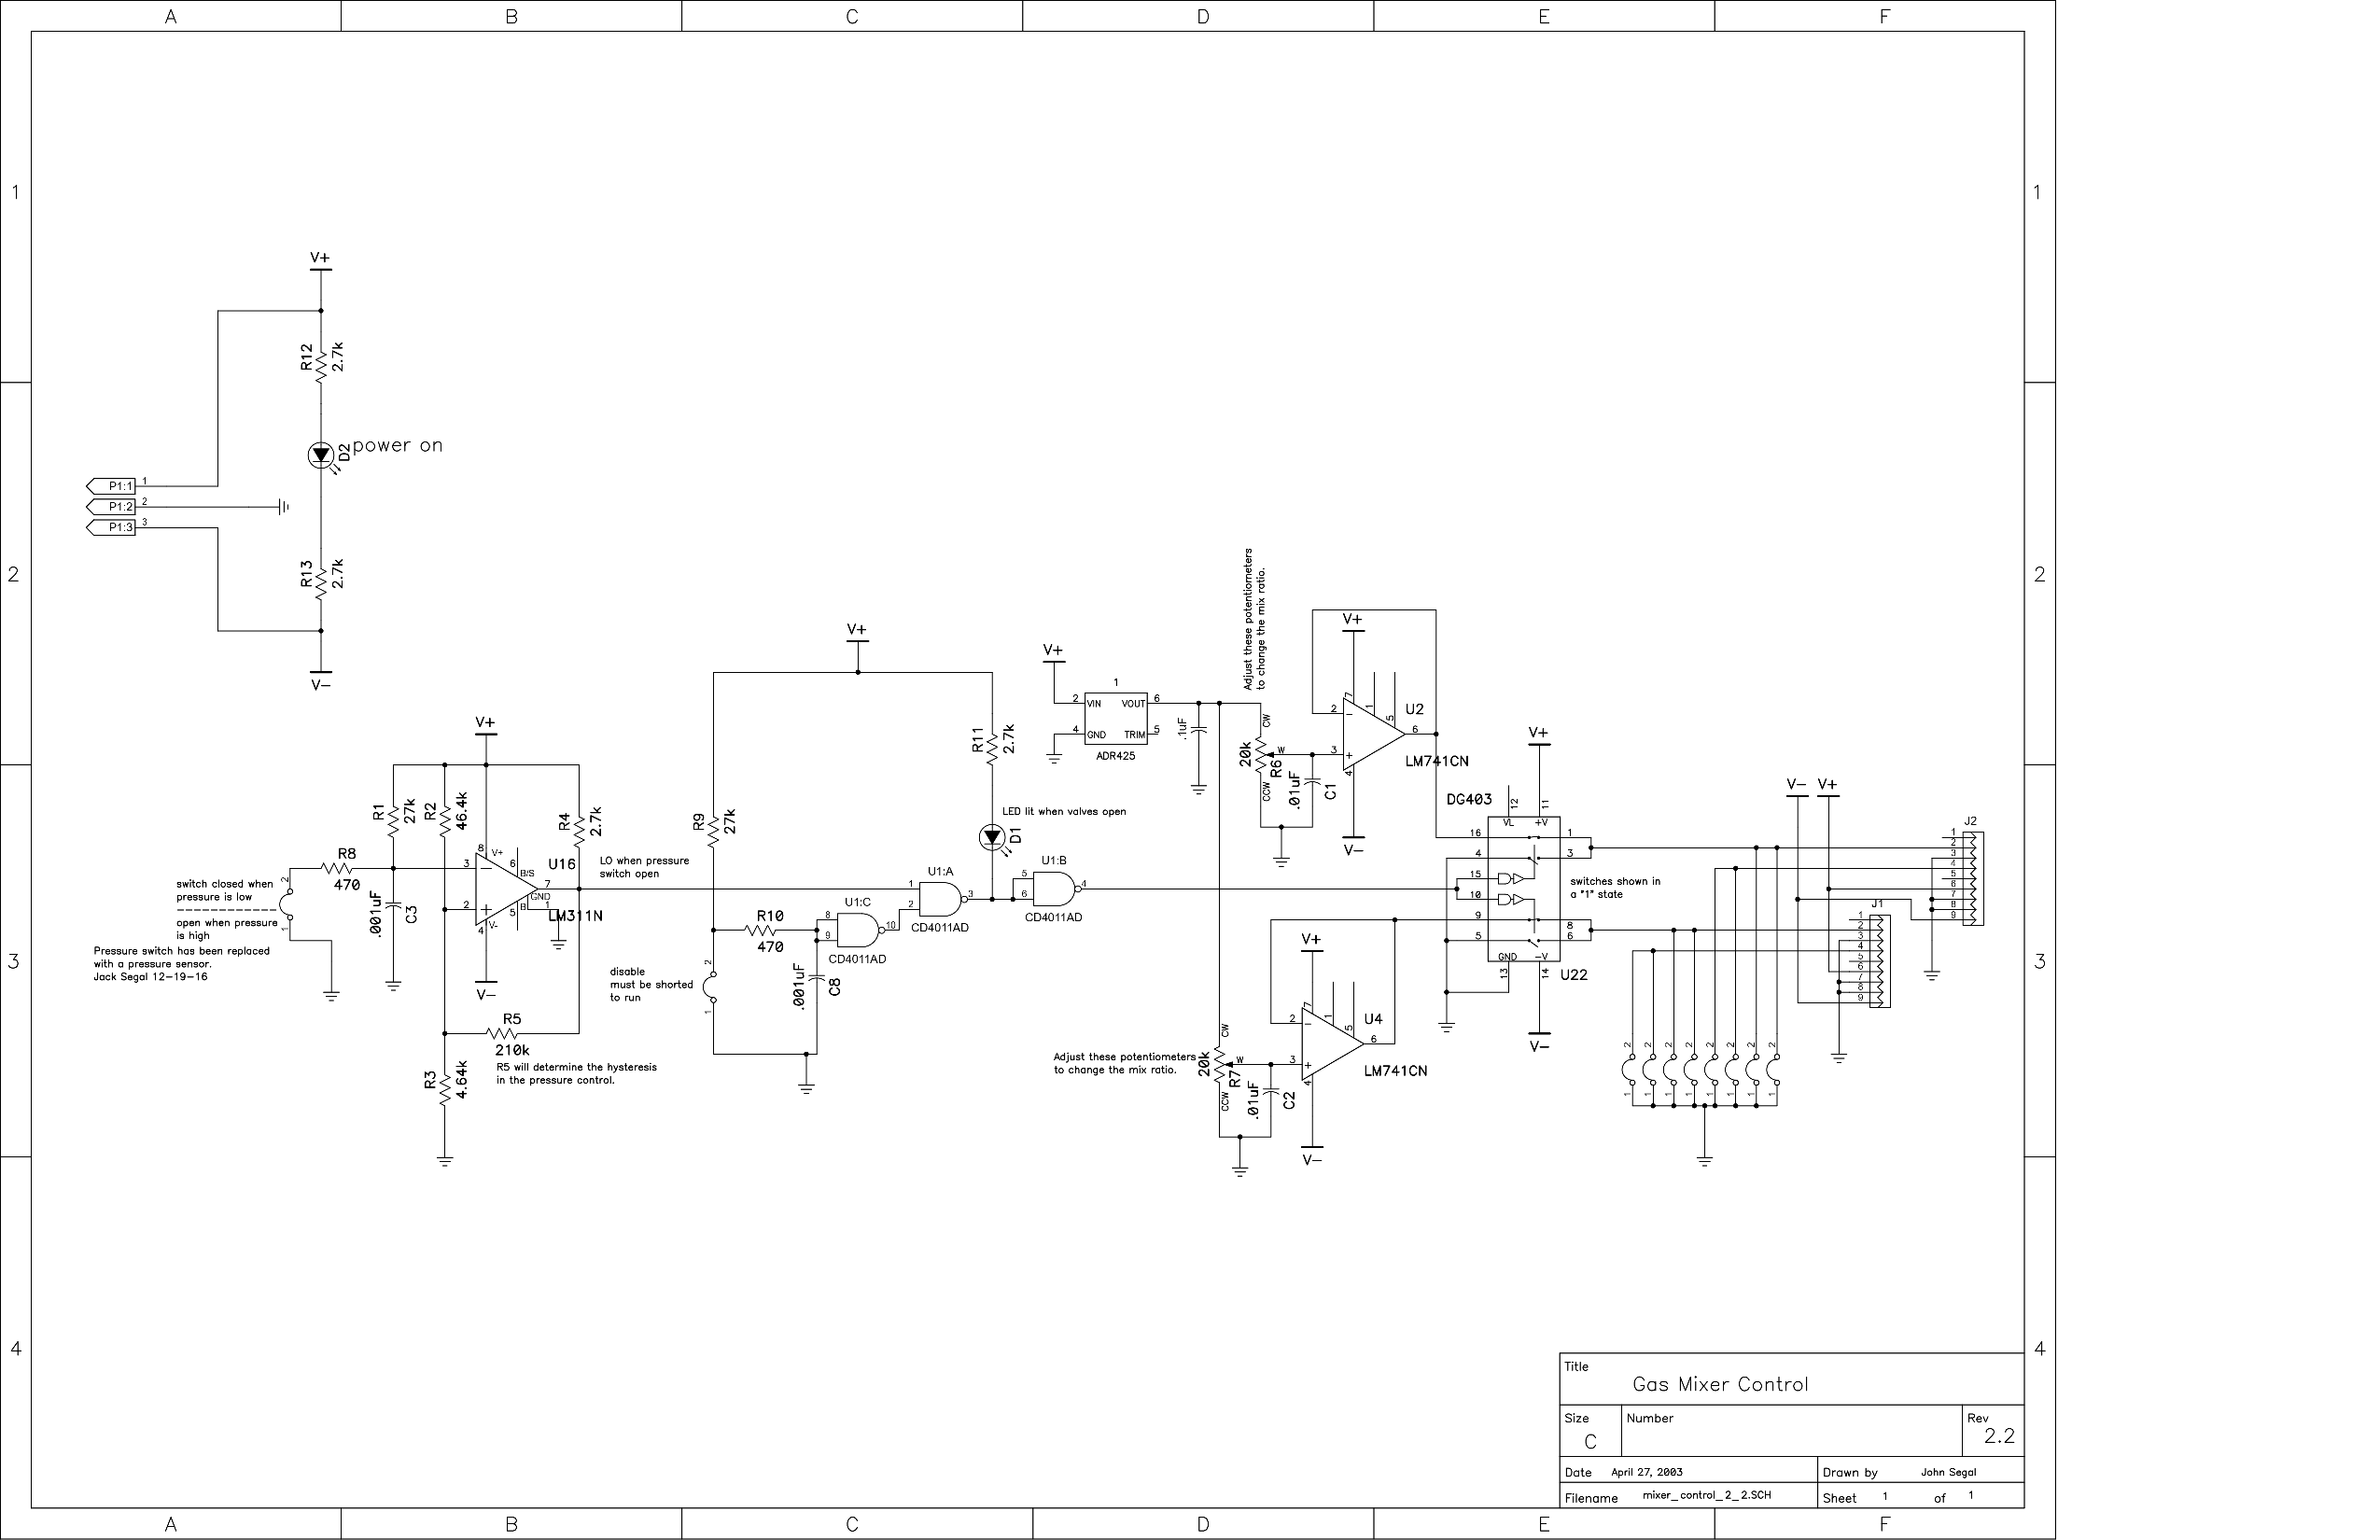
\includegraphics[angle=0,width=0.9\textwidth,clip]{MixingControl.pdf}
\caption{The regulator for the nitrogen bottles used for bottle switching.}
\label{fig:SwitchingElectronics}
\end{center}
\end{figure}



\begin{safetyen}{0}{0}
\infolevone{\section{Safety Information}}
\label{sec:hrs-det-gasalarms}


\subsection{Hazards}

None of the gases that are used are flammable. So, no fire hazard related to the gas. However, the gas bottles
are under high pressure and can become missiles.
 One can get injured if the gas bottles are not handled properly while transferring from the storage rack to the rack inside the shed.

The liquid nitrogen dewar possesses hazards related to the cryogenic system.
Also, these gases are colorless and odorless, which can cause asphyxiation if not handled properly in a closed area. 
\subsection{Mitigations}

People who are handling the gas system should take the SAF130AU and understand the risks associated with a high-pressure system. 
The gas bottles are in the gas sheds which are in the open air with adequate ventilation.
The gas bottles are always located in a gas rack with a securing chain so that they can not fall.
 People handling cylinders should wear leather safety gloves and safety shoes when handling cylinders. While moving cylinders, even for short distances, use a cart designed to transport cylinders.
 

While working with the dewar, one needs to be careful of handling the valves on the top of the dewar. It can cause cold burns. 
Use a safety glass and cryogenic compatible gloves.

\subsection{Responsible Personnel}

Maintenance of the gas systems is routinely performed by the Hall A
technical staff.  Shift personnel are not expected to be responsible
for maintaining the detector gas systems (see Table \ref{tab:gas:personnel}  
for the names of persons to be contacted in case of problems). 

\begin{namestab}{tab:gas:personnel}{Gas for wire chambers: authorized personnel}{%
      Responsible personnel for detector gas system.}
  \TechonCall{\em Contact}
  \IbrahimAlbayrak{}
  \LarsGustavson{}
 % \JackSegal{}
  \ChandanGhosh{}
\end{namestab}
\end{safetyen}
